\documentclass[18pt,xcolor=table]{beamer}

%!TEX root = ./main.tex
\usepackage {bbm}
\usepackage {textpos}
\usepackage {tikz}
\usepackage {graphicx}


\definecolor{blue1}{RGB}{176,196,222 }
\definecolor{blue2}{RGB}{54,100,139}

\definecolor{grey1}{RGB}{139,139,131}
\definecolor{grey2}{RGB}{235,235,235}

\definecolor{black1}{RGB}{50,50,50}

\mode<presentation>
{
  % \usetheme{Pittsburgh}   
  %\usetheme{Boadilla}  
\usetheme{Madrid}  
  \usefonttheme[onlymath]{serif}
  \setbeamertemplate{items}[circle] 
  \setbeamertemplate{sections/subsections in toc}[circle]
  \setbeamercovered{invisible}
  \setbeamertemplate{navigation symbols}{}
% \usecolortheme{seahorse}
%
%  % Color Theme 
  \setbeamercolor{normal text}{bg=white,fg=black1} %All standard text
  \setbeamercolor{structure}{fg=blue2} %% Table of Contents 

  \setbeamercolor*{frametitle}{fg=black1,bg=grey2} % Frame title colors
%  \setbeamerfont{frametitle}{series=\bfseries}
  \setbeamercolor*{framesubtitle}{fg=blue2} % Frame subtitle color

  \setbeamercolor*{palette primary}{use=structure,fg=black1, bg=grey2} %right bottom
  \setbeamercolor*{palette secondary}{use=structure,bg=blue1} %middle bottom
  \setbeamercolor*{palette tertiary}{use=structure,bg=blue2,fg=grey2} %left bottom

  \setbeamercolor*{block body}{fg=black1,bg=blue1!10} % Color of blocks
  \setbeamercolor*{block title}{parent=structure,fg=black1,bg=blue1} % Block Titles
  \setbeamercolor{alerted text}{fg=blue2!85!black,} % Alerted Text (ie. highlight with \alert)
  \setbeamerfont{alerted text}{series=\bfseries}

  % not sure what these do.
  \setbeamercolor{item projected}{use=item,fg=black1,bg=item.fg!35}
  \setbeamercolor*{block title alerted}{parent=alerted text,bg=black1!15}
  \setbeamercolor*{block title example}{parent=example text,bg=black1!15}
  \setbeamerfont{framesubtitle}{size=\small}
}

\makeatletter
\setbeamertemplate{footline}
{
  \leavevmode%
    \hbox{%
      \begin{beamercolorbox}[wd=.333333\paperwidth,ht=2.25ex,dp=1ex,center]{author in head/foot}%
        \usebeamerfont{author in head/foot}\insertshortauthor%~~\beamer@ifempty{\insertshortinstitute}{}{(\insertshortinstitute)}
      \end{beamercolorbox}%
        \begin{beamercolorbox}[wd=.333333\paperwidth,ht=2.25ex,dp=1ex,center]{title in head/foot}%
        \usebeamerfont{title in head/foot}\insertshorttitle
        \end{beamercolorbox}%
        \begin{beamercolorbox}[wd=.333333\paperwidth,ht=2.25ex,dp=1ex,right]{date in head/foot}%
        \usebeamerfont{date in head/foot}\insertshortdate{}\hspace*{2em}
        \insertframenumber{} / \inserttotalframenumber\hspace*{2ex} 
      \end{beamercolorbox}}%
        \vskip0pt%
}
\makeatother

%\usepackage{kerkis}
\usepackage{helvet} 
\usepackage[T1]{fontenc}
\usepackage[protrusion=true,expansion=true]{microtype}
\usepackage{amsmath}

\renewcommand*{\thefootnote}{\fnsymbol{footnote}}


\pgfdeclareimage[height=1.5cm]{logo}{./logos/hd_logo}
\pgfdeclareimage[height=0.8cm]{small_logo}{./logos/hd_logo}

\AtBeginSection[] { 
  \begin{frame}[plain] 
    \frametitle{\bf Outline:}
    \framesubtitle{~~} 
    \tableofcontents[currentsection] 
  \end{frame} 
  \addtocounter{framenumber}{-1} 
} 

\setbeamercovered{transparent}

%%%%%%%%%%%%%%%%%%%%%%%
% user-defined commands
%%%%%%%%%%%%%%%%%%%%%%%
%!TEX root = ../main.tex


\newcommand{\beq}{\begin{equation}}
\newcommand{\eeq}{\end{equation}}

\newcommand{\eq}[1]{\begin{align*}#1\end{align*}}

\newcommand{\bfi}{\begin{figure}}
\newcommand{\efi}{\end{figure}}

\newcommand{\icg}{\includegraphics}

\newcommand{\bdm}{\begin{displaymath}}
\newcommand{\edm}{\end{displaymath}}

\newcommand{\beqa}{\begin{eqnarray}}
\newcommand{\eeqa}{\end{eqnarray}}

\newcommand{\beqas}{\begin{eqnarray*}}
\newcommand{\eeqas}{\end{eqnarray*}}

\newcommand{\barr}{\begin{array}}
\newcommand{\earr}{\end{array}}

\newcommand{\bit}{\begin{itemize}}
\newcommand{\eit}{\end{itemize}}

\newcommand{\qq}[1]{\qquad \mbox{#1} \qquad}

\def\hyph{-\penalty0\hskip0pt\relax}

% Tikz
\definecolor{blue1}{RGB}{176,196,222 }
\definecolor{blue2}{RGB}{54,100,139}
\definecolor{grey1}{RGB}{139,139,131}
\definecolor{grey2}{RGB}{235,235,235}
\definecolor{black1}{RGB}{50,50,50}


%Spaces
\newcommand{\Sp}[1]{{\cal #1}}
%
\newcommand{\sA}{\Sp{A}}
\newcommand{\sB}{\Sp{B}}
\newcommand{\sC}{\Sp{C}}
\newcommand{\sD}{\Sp{D}}
\newcommand{\sE}{\Sp{E}}
\newcommand{\sF}{\Sp{F}}
\newcommand{\sG}{\Sp{G}}
\newcommand{\sH}{\Sp{H}}
\newcommand{\sI}{\Sp{I}}
\newcommand{\sJ}{\Sp{J}}
\newcommand{\sK}{\Sp{K}}
\newcommand{\sL}{\Sp{L}}
\newcommand{\sM}{\Sp{M}}
\newcommand{\sN}{\Sp{N}}
\newcommand{\sO}{\Sp{O}}
\newcommand{\sP}{\Sp{P}}
\newcommand{\sQ}{\Sp{Q}}
\newcommand{\sR}{\Sp{R}}
\newcommand{\sS}{\Sp{S}}
\newcommand{\sT}{\Sp{T}}
\newcommand{\sU}{\Sp{U}}
\newcommand{\sV}{\Sp{V}}
\newcommand{\sW}{\Sp{W}}
\newcommand{\sX}{\Sp{X}}
\newcommand{\sY}{\Sp{Y}}
\newcommand{\sZ}{\Sp{Z}}

%Vectors
\newcommand{\V}[1]{{\bf #1}}
%
\newcommand{\va}{\V{a}}
\newcommand{\vb}{\V{b}}
\newcommand{\vc}{\V{c}}
\newcommand{\vd}{\V{d}}
\newcommand{\ve}{\V{e}}
\newcommand{\vf}{\V{f}}
\newcommand{\vg}{\V{g}}
\newcommand{\vh}{\V{h}}
\newcommand{\vi}{\V{i}}
\newcommand{\vj}{\V{j}}
\newcommand{\vk}{\V{k}}
\newcommand{\vl}{\V{l}}
\newcommand{\vm}{\V{m}}
\newcommand{\vn}{\V{n}}
\newcommand{\vo}{\V{o}}
\newcommand{\vp}{\V{p}}
\newcommand{\vq}{\V{q}}
\newcommand{\vr}{\V{r}}
\newcommand{\vs}{\V{s}}
\newcommand{\vt}{\V{t}}
\newcommand{\vu}{\V{u}}
\newcommand{\vv}{\V{v}}
\newcommand{\vw}{\V{w}}
\newcommand{\vx}{\V{x}}
\newcommand{\vy}{\V{y}}
\newcommand{\vz}{\V{z}}

\newcommand{\vA}{\V{A}}
\newcommand{\vB}{\V{B}}
\newcommand{\vC}{\V{C}}
\newcommand{\vD}{\V{D}}
\newcommand{\vE}{\V{E}}
\newcommand{\vF}{\V{F}}
\newcommand{\vG}{\V{G}}
\newcommand{\vH}{\V{H}}
\newcommand{\vI}{\V{I}}
\newcommand{\vJ}{\V{J}}
\newcommand{\vK}{\V{K}}
\newcommand{\vL}{\V{L}}
\newcommand{\vM}{\V{M}}
\newcommand{\vN}{\V{N}}
\newcommand{\vO}{\V{O}}
\newcommand{\vP}{\V{P}}
\newcommand{\vQ}{\V{Q}}
\newcommand{\vR}{\V{R}}
\newcommand{\vS}{\V{S}}
\newcommand{\vT}{\V{T}}
\newcommand{\vU}{\V{U}}
\newcommand{\vV}{\V{V}}
\newcommand{\vW}{\V{W}}
\newcommand{\vX}{\V{X}}
\newcommand{\vY}{\V{Y}}
\newcommand{\vZ}{\V{Z}}

\newcommand{\vone}{\V{1}}
\newcommand{\vzero}{\V{0}}
\newcommand{\B}{\V{B}}
\newcommand{\E}{\V{E}}
\newcommand{\Er}{\V{E}_r}
\newcommand{\Es}{\V{E}_s}
\newcommand{\un}{\hat{\vn}}



%Vectors
\newcommand{\T}[1]{\underline{\bf #1}}
%
\newcommand{\ta}{\T{a}}
\newcommand{\tb}{\T{b}}
\newcommand{\tc}{\T{c}}
%\newcommand{\td}{\T{d}}
\newcommand{\te}{\T{e}}
\newcommand{\tf}{\T{f}}
\newcommand{\tg}{\T{g}}
%\newcommand{\th}{\T{h}}
\newcommand{\ti}{\T{i}}
\newcommand{\tj}{\T{j}}
\newcommand{\tk}{\T{k}}
\newcommand{\tl}{\T{l}}
\newcommand{\tm}{\T{m}}
\newcommand{\tn}{\T{n}}
%\newcommand{\to}{\T{o}}
\newcommand{\tp}{\T{p}}
\newcommand{\tq}{\T{q}}
\newcommand{\tr}{\T{r}}
\newcommand{\ts}{\T{s}}
%\newcommand{\tt}{\T{t}}
\newcommand{\tu}{\T{u}}
\newcommand{\tv}{\T{v}}
\newcommand{\tw}{\T{w}}
\newcommand{\tx}{\T{x}}
\newcommand{\ty}{\T{y}}
\newcommand{\tz}{\T{z}}

\newcommand{\tA}{\T{A}}
\newcommand{\tB}{\T{B}}
\newcommand{\tC}{\T{C}}
\newcommand{\tD}{\T{D}}
\newcommand{\tE}{\T{E}}
\newcommand{\tF}{\T{F}}
\newcommand{\tG}{\T{G}}
\newcommand{\tH}{\T{H}}
\newcommand{\tI}{\T{I}}
\newcommand{\tJ}{\T{J}}
\newcommand{\tK}{\T{K}}
\newcommand{\tL}{\T{L}}
\newcommand{\tM}{\T{M}}
\newcommand{\tN}{\T{N}}
\newcommand{\tO}{\T{O}}
\newcommand{\tP}{\T{P}}
\newcommand{\tQ}{\T{Q}}
\newcommand{\tR}{\T{R}}
\newcommand{\tS}{\T{S}}
\newcommand{\tT}{\T{T}}
\newcommand{\tU}{\T{U}}
\newcommand{\tV}{\T{V}}
\newcommand{\tW}{\T{W}}
\newcommand{\tX}{\T{X}}
\newcommand{\tY}{\T{Y}}
\newcommand{\tZ}{\T{Z}}

\newcommand{\tone}{\T{1}}
\newcommand{\tzero}{\T{0}}

%Matrix
\newcommand{\M}[1]{{\mathbb #1}}
%
\newcommand{\mA}{\M{A}}
\newcommand{\mB}{\M{B}}
\newcommand{\mC}{\M{C}}
\newcommand{\mD}{\M{D}}
\newcommand{\mE}{\M{E}}
\newcommand{\mF}{\M{F}}
\newcommand{\mG}{\M{G}}
\newcommand{\mH}{\M{H}}
\newcommand{\mI}{\M{I}}
\newcommand{\mJ}{\M{J}}
\newcommand{\mK}{\M{K}}
\newcommand{\mL}{\M{L}}
\newcommand{\mM}{\M{M}}
\newcommand{\mN}{\M{N}}
\newcommand{\mO}{\M{O}}
\newcommand{\mP}{\M{P}}
\newcommand{\mQ}{\M{Q}}
\newcommand{\mR}{\M{R}}
\newcommand{\mS}{\M{S}}
\newcommand{\mT}{\M{T}}
\newcommand{\mU}{\M{U}}
\newcommand{\mV}{\M{V}}
\newcommand{\mW}{\M{W}}
\newcommand{\mX}{\M{X}}
\newcommand{\mY}{\M{Y}}
\newcommand{\mZ}{\M{Z}}

\newcommand{\mzero}{\M{0}}
\newcommand{\mone}{\M{1}}

% Derivatives
\newcommand{\pd}[2]{\frac{\partial #1}{\partial #2}}
\newcommand{\ppd}[2]{\frac{\partial^2 #1}{\partial #2^2}}
\newcommand{\td}[2]{\frac{\mathrm{d} #1}{\mathrm{d} #2}}

\newcommand{\px}{ \partial_{x} }
\newcommand{\py}{ \partial_{y} }
\newcommand{\pz}{ \partial_{z} }
\newcommand{\pt}{ \partial_{t} }
\newcommand{\ptt}{ \partial_{tt} }

\newcommand{\Div}[1]{\nabla \cdot #1}
\newcommand{\Curl}[1]{\nabla \times #1}
\newcommand{\Ctwo}[1]{\nabla_2 \times #1}
\newcommand{\Grad}[1]{\nabla #1}
\newcommand{\Gperp}[1]{\nabla^\perp #1}
\newcommand{\Lap}[1]{\Delta #1}

%integral d
\newcommand{\dd}[0]{\, \mathrm{d}}

% common discrete quantities
\newcommand{\dt}[0]{\delta t}

% physical variables
\newcommand{\eps}[0]{\epsilon_0}
\newcommand{\mus}[0]{\mu_0}
\newcommand{\boltz}[0]{\kappa_B}
\newcommand{\s}[0]{\alpha}
\newcommand{\vths}[0]{v_{th_\s}}
\newcommand{\vthe}[0]{v_{th_e}}
\newcommand{\vthi}[0]{v_{th_i}}
\newcommand{\Om}[0]{\Omega}
\newcommand{\bdOm}{\partial \Omega}

% bracketing
\newcommand{\inner}[2]{\langle #1, #2 \rangle}
\newcommand{\lb}[0]{\left[}
\newcommand{\rb}[0]{\right]}
\newcommand{\parn}[1]{\left( #1 \right)}
\newcommand{\la}{\langle}
\newcommand{\ra}{\rangle}
\newcommand{\lcb}{\left\{}
\newcommand{\rcb}{\right\}}

\newcommand{\mathAnd}{\,\,\mbox{and}\,\,}
\newcommand{\mathOn}{\,\,\mbox{on}\,\,}

\newcommand{\h}{\hat}
\newcommand{\wh}{\widehat}
%\newcommand{\ul}{\underline}

% math operators
\DeclareMathOperator{\Trace}{trace}
\DeclareMathOperator{\Supp}{supp}
\DeclareMathOperator{\Span}{span}
\DeclareMathOperator{\floor}{floor}
\DeclareMathOperator{\diam}{diam}
\DeclareMathOperator{\ceil}{ceil}
\DeclareMathOperator*{\argmin}{arg\,min}


\newcommand{\red}[1]{\textcolor{red}{#1}}
%added macro definitions here

\usepackage{tikz}
\usepackage{tabularx}
\usetikzlibrary{decorations.markings}
\usetikzlibrary{arrows,positioning} 

\usepackage{cancel}
\usepackage{hyperref}
\usepackage{caption}
\usepackage{subcaption}
\usepackage[]{algorithm}
\usepackage{algpseudocode}
\captionsetup{compatibility=false}


\title[Multigrid]{Introduction to Multigrid Methods}
\subtitle{Day 5: parallel AMG}
\author[Mitchell]{Wayne Mitchell}
\institute{\pgfuseimage{logo}\\Universit\"at Heidelberg\\Institut f\"ur Technische Informatik}
\date[]{\alert{}}


\begin{document}
%!TEX root = ./main.tex
\tikzstyle{block} = [rectangle, draw, rounded corners, shade, top color=white, text width=5em,
  bottom color=blue!50!black!20, draw=blue!40!black!60, very thick, text centered, minimum height=4em]
  \tikzstyle{line} = [draw, -latex']
  \tikzstyle{cloud} = [draw, ellipse,top color=white, bottom color=red!20, node distance=2cm, minimum height=2em]

  \frame{\titlepage}

  \addtobeamertemplate{frametitle}{}{%
      \begin{textblock*}{100mm}(0.9\textwidth,-0.88cm)
    \pgfuseimage{small_logo}
    \end{textblock*}
  }

\AtBeginSection[] { 
  \begin{frame}[t]
    \frametitle{\bf Outline:}
    \framesubtitle{~~} 
    \tableofcontents[currentsection] 
  \end{frame} 
  \addtocounter{framenumber}{-1} 
} 

\let\tempone\itemize
\let\temptwo\enditemize
\renewenvironment{itemize}{\tempone\addtolength{\itemsep}{0.5\baselineskip}}{\temptwo}

\DeclareRobustCommand{\Chi}{\raisebox{2pt}{$\chi$}}
%%%%%%%%%%%%%%%%%%%%%%%%%%%%%%%%%%%%%%%%%%%%%%%%%%%%%%%%%%%%%%%%%%%%%%%%%%%%%%%%

% Slide
\begin{frame}{}
\begin{block}{Day 5 Goals}
\bit
\item Session 1:
\bit
\item Development of \emph{hypre} BoomerAMG
\eit
\item Session 2:
\bit
\item Algebraic multigrid domain decomposition (AMG-DD)
\eit
\item Session 3:
\bit
\item Discussion and hands-on examples
\eit
\eit
\end{block}
\end{frame}

\begin{frame}
\frametitle{\bf Outline:}
\framesubtitle{~~}
\tableofcontents
\end{frame}

%%%%%%%%%%%%%%%%%%%%%%%%%%%%%%%%%%%%%%%%%%%%%%%%%%%%%%%%%%%%%%%%%%%%%%%%%%%%%%%%

\section{Development of \emph{hypre}}

\begin{frame}{Development of \emph{hypre}}
\begin{block}{Parallel AMG}
\bit
\item Recall that the appeal of multigrid is its $O(N)$ computational cost
\item Want to use multigrid for \emph{very} large problems on large parallel machines
\item Efficient parallelization of multigrid, particularly AMG, is non-trivial
\eit
\end{block}
\end{frame}

\begin{frame}{Development of \emph{hypre}}
\begin{block}{Parallel AMG}
\bit
\item AMG setup: need parallel coarsening algorithms and corresponding interpolation strategies
\item AMG solve: need parallel smoothers
\eit
\end{block}
\end{frame}

\begin{frame}{Development of \emph{hypre}}
\begin{block}{AMG coarsening in parallel}
\bit
\item Henson and Yang. BoomerAMG: A parallel algebraic multigrid solver and preconditioner. Appl. Num. Math. 2002.
\item Classical coloring algorithm is sequential in nature
\item First attempts at parallel coarsening:
\bit
\item Cleary-Luby-Jones-Plassman (CLJP) coarsening
\item Parallel Ruge-St\"uben coarsening
\item Falgout coarsening
\eit
\eit
\end{block}
\end{frame}

\begin{frame}{Development of \emph{hypre}}
\begin{block}{CLJP coarsening}
\bit
\item Based on parallel graph partitioning
\eit
\end{block}
\end{frame}

\begin{frame}{Development of \emph{hypre}}
\begin{block}{}
\bit
\item 
\eit
\end{block}
\end{frame}


% References:
% Henson and Yang. BoomerAMG: A parallel algebraic multigrid solver and preconditioner. Appl. Num. Math. 2002.
% De Sterck, Yang, and Heys. Reducing complexity in parallel algebraic multigrid preconditioners. SIAM J. Mat. Anal. Appl. 2006.
% De Sterck, Falgout, Nolting, and Yang. Distance-Two Interpolation for Parallel Algebraic Multigrid. Numer. Lin. Alg. Appl. 2007.
% Baker, Falgout, Kolev, and Yang. Multigrid smoothers for ultra-parallel computing. SIAM J. Sci. Comp. 2011.


% Include stuff on AmgX? At least a mention...

% Briefly include other ideas for reducing complexity: additive variants, non-galerkin sparsification, etc.

%%%%%%%%%%%%%%%%%%%%%%%%%%%%%%%%%%%%%%%%%%%%%%%%%%%%%%%%%%%%%%%%%%%%%%%%%%%%%%%%

\section{Algebraic multigrid domain decomposition (AMG-DD)}

% Slide 
\begin{frame}{MotivationAlgebraic multigrid domain decomposition (AMG-DD)}
\begin{block}{Communication-limited AMG}
\begin{itemize}
\item Even current best practices can still yield severely communication-limited AMG algorithms due to coarse-grid complexity
\end{itemize}
\end{block}

\begin{center}
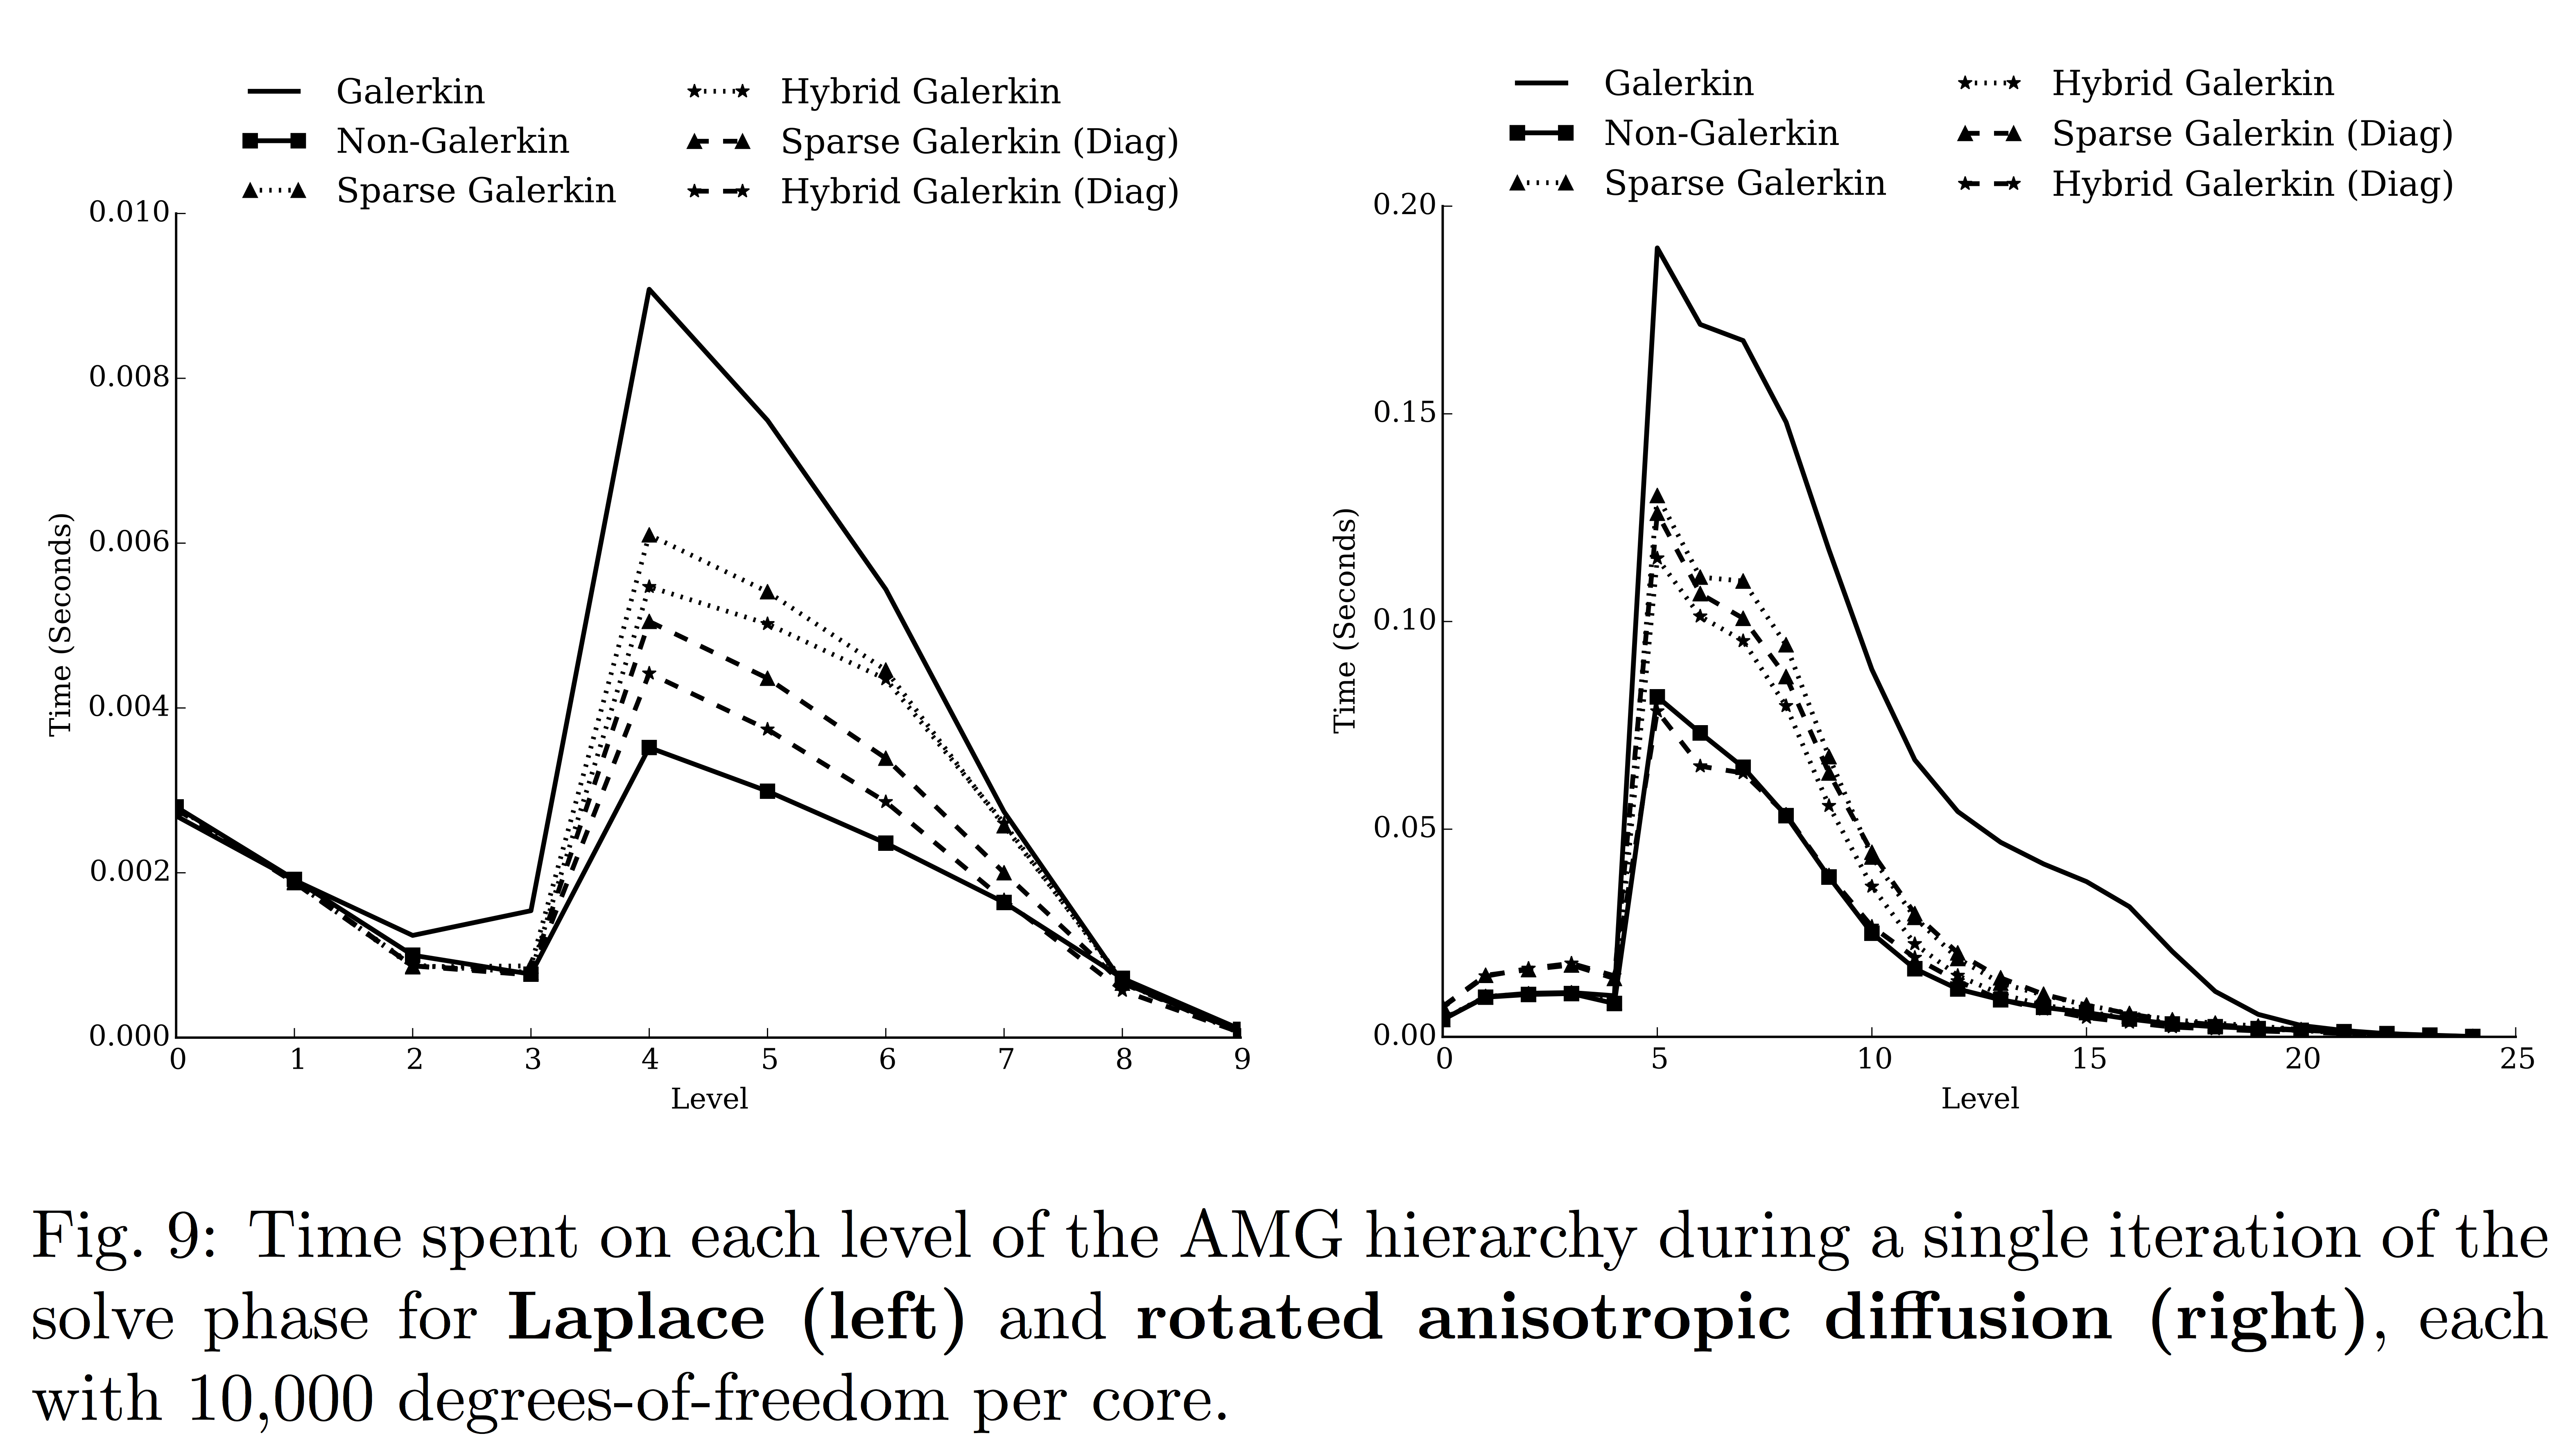
\includegraphics[width=0.7\textwidth]{../figures/nonGalerkinFigure}
\end{center}
\tiny{Figure credit: Bienz, Falgout, Gropp, Olson, and Schroder. Reducing parallel communication in algebraic multigrid through sparsification. SIAM J. Sci. Comp. 2016.}

\end{frame}

% Slide 
% This is where AMG-DD comes in.
\begin{frame}{Algebraic multigrid domain decomposition (AMG-DD)}
\begin{block}{Algebraic multigrid domain decomposition (AMG-DD)}
\begin{itemize}
\item Rather than continue modifying components of AMG, design a new algorithm altogether
\item Algebraic multigrid domain decomposition (AMG-DD) utilizes 
\item AMG-DD seeks to reduce communication cost by
\begin{itemize}
\item Enabling more independent computation in between communications
\item Trading moderately more computation for significantly less communication
\end{itemize}
\end{itemize}
\end{block}

\end{frame}

% Slide
\begin{frame}{Algebraic multigrid domain decomposition (AMG-DD)}
\begin{block}{Composite Grids}
\begin{itemize}
\item Each processor solves a representation of the global problem
\item Composite grids resemble adaptively refined meshes but are built using an existing AMG hierarchy
\end{itemize}
\end{block}
\centering
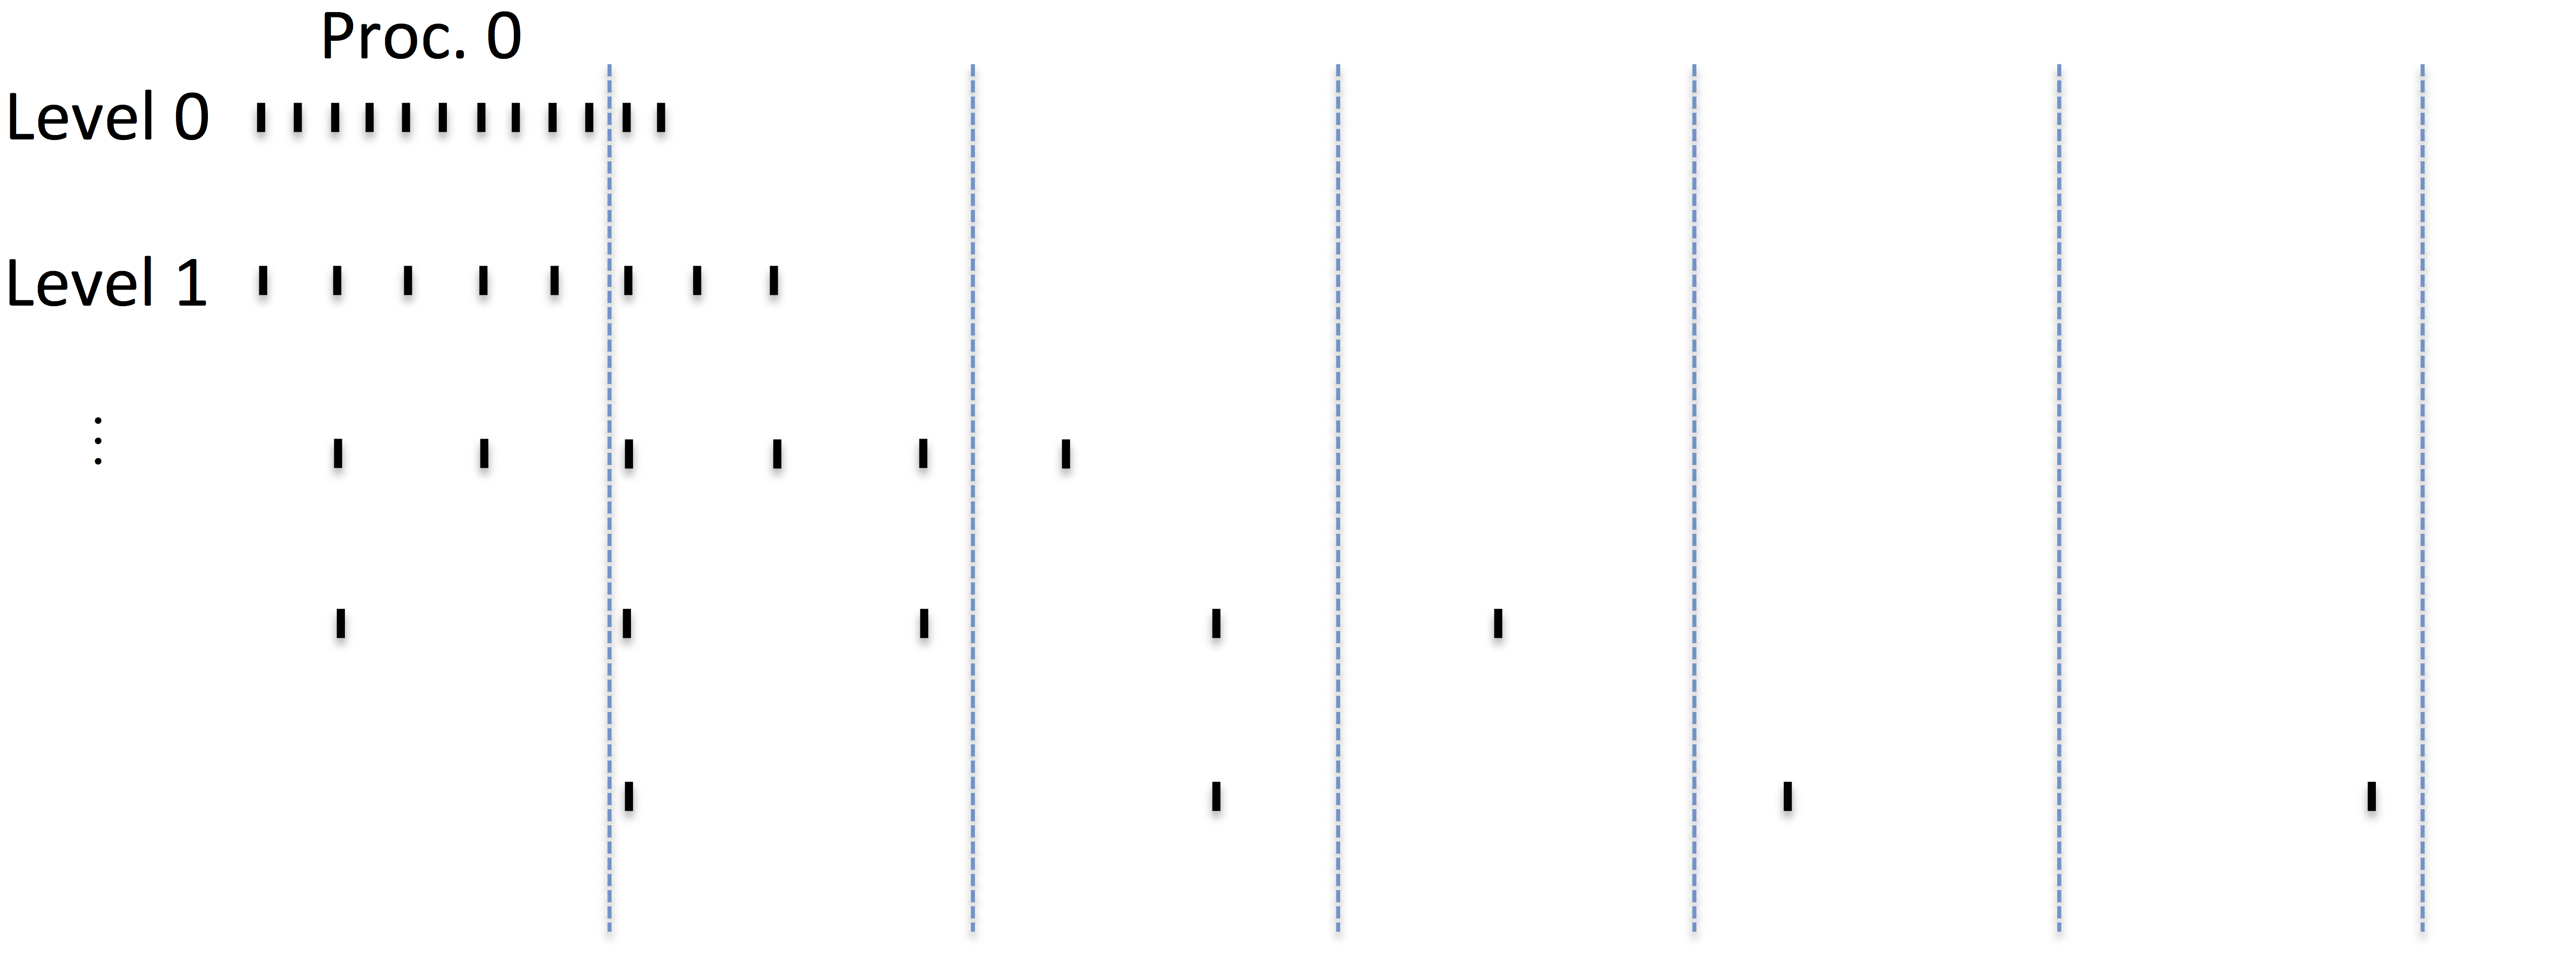
\includegraphics[width=\textwidth]{../figures/compGridCreation1D13}
\end{frame}

% Slide
% Composite grids are constructed as follows. We first choose a value called the padding, for this example we'll use padding 2. Then starting on the fine grid, add all points withing distance 2 through the stencil of the matrix. Then coarsen that set and add those points on the next level to the composite grid. Now simply repeat this process all the way down.
\begin{frame}{Algebraic multigrid domain decomposition (AMG-DD)}
\begin{block}{}
Composite grid creation in 1D with padding 2
\end{block}
\vspace{1 cm}
\only<1>{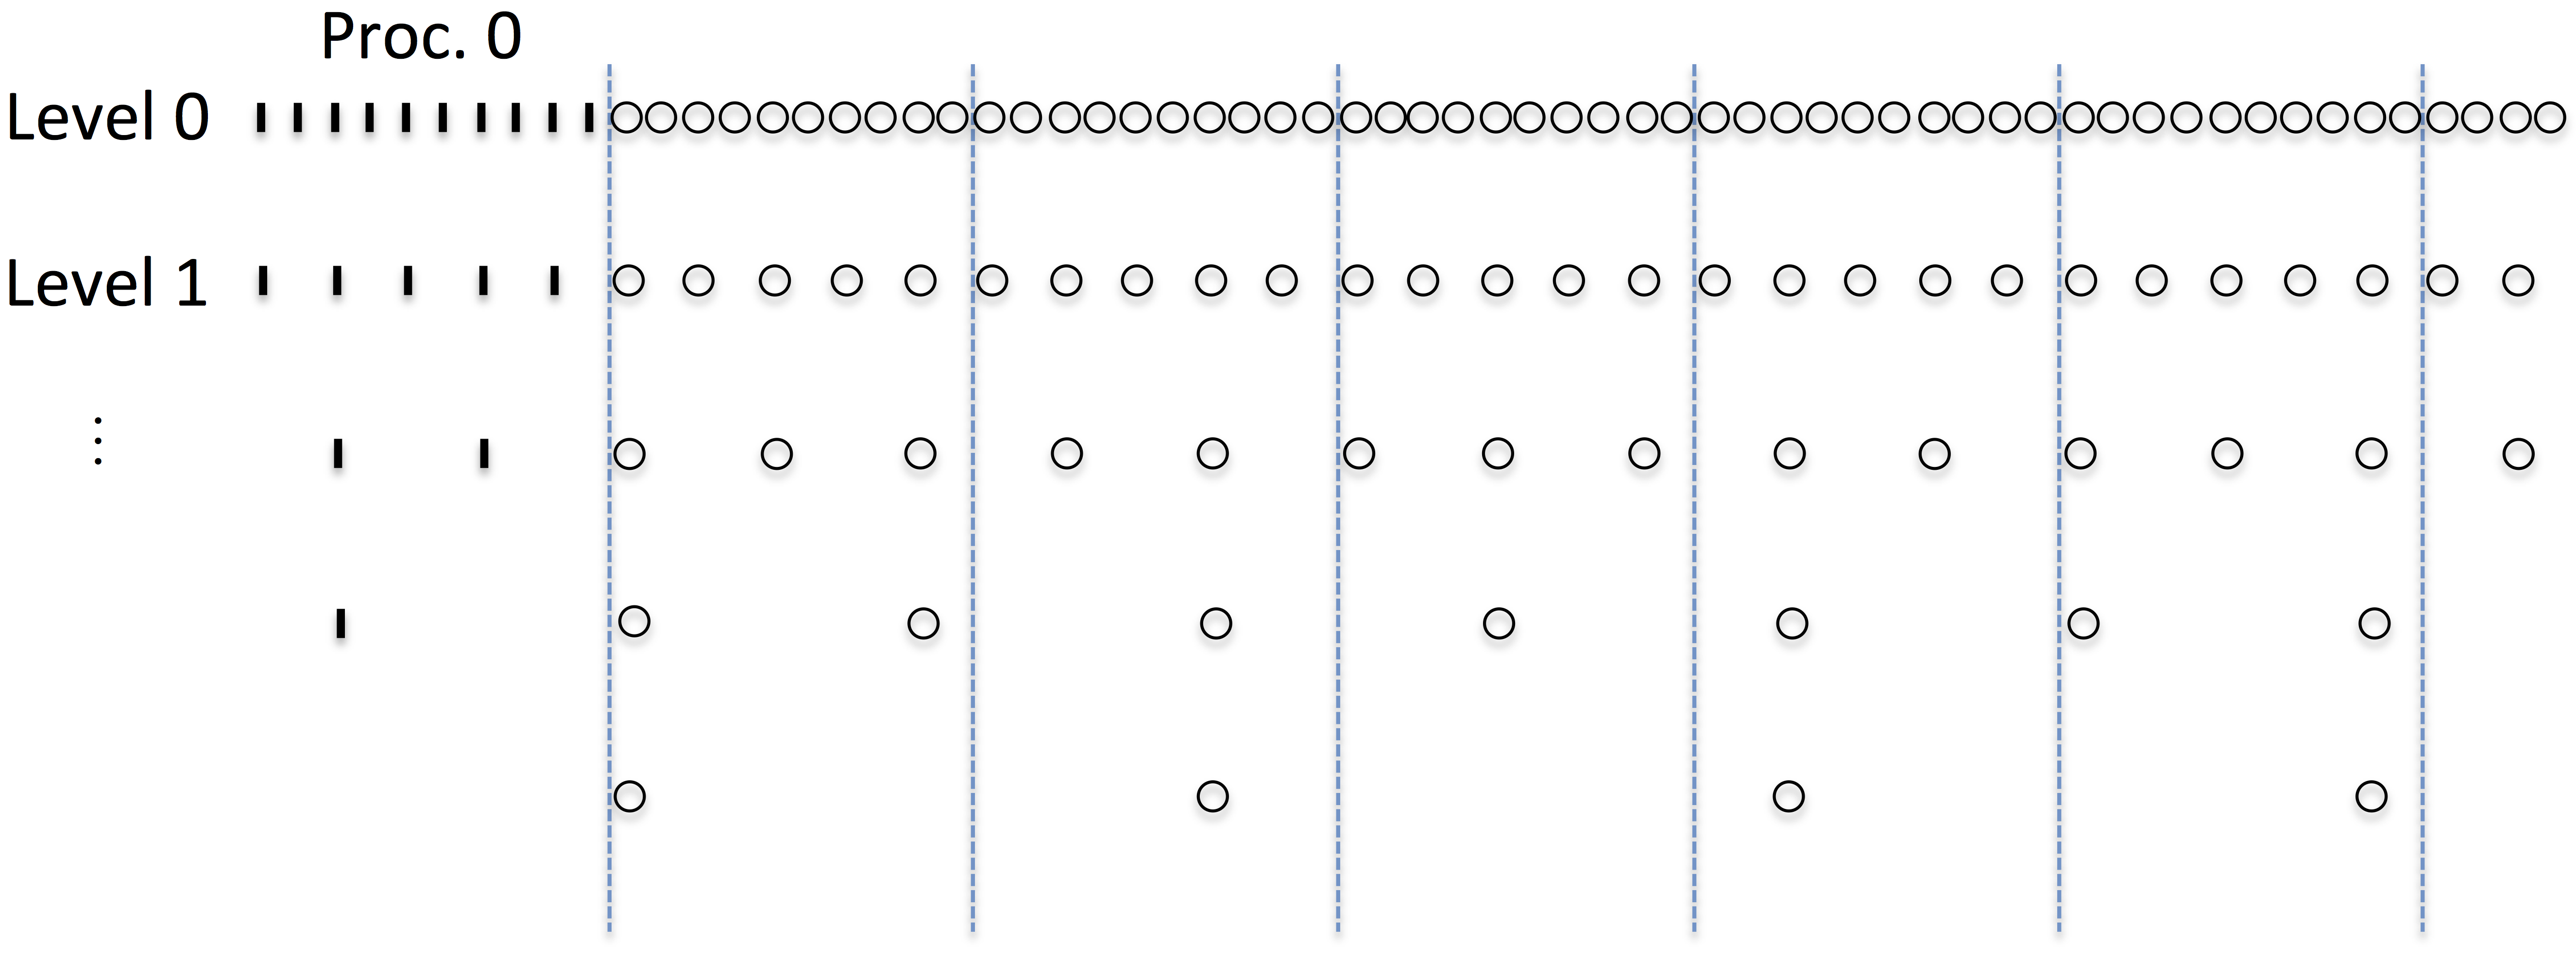
\includegraphics[width=\textwidth]{../figures/compGridCreation1D3}}
\only<2>{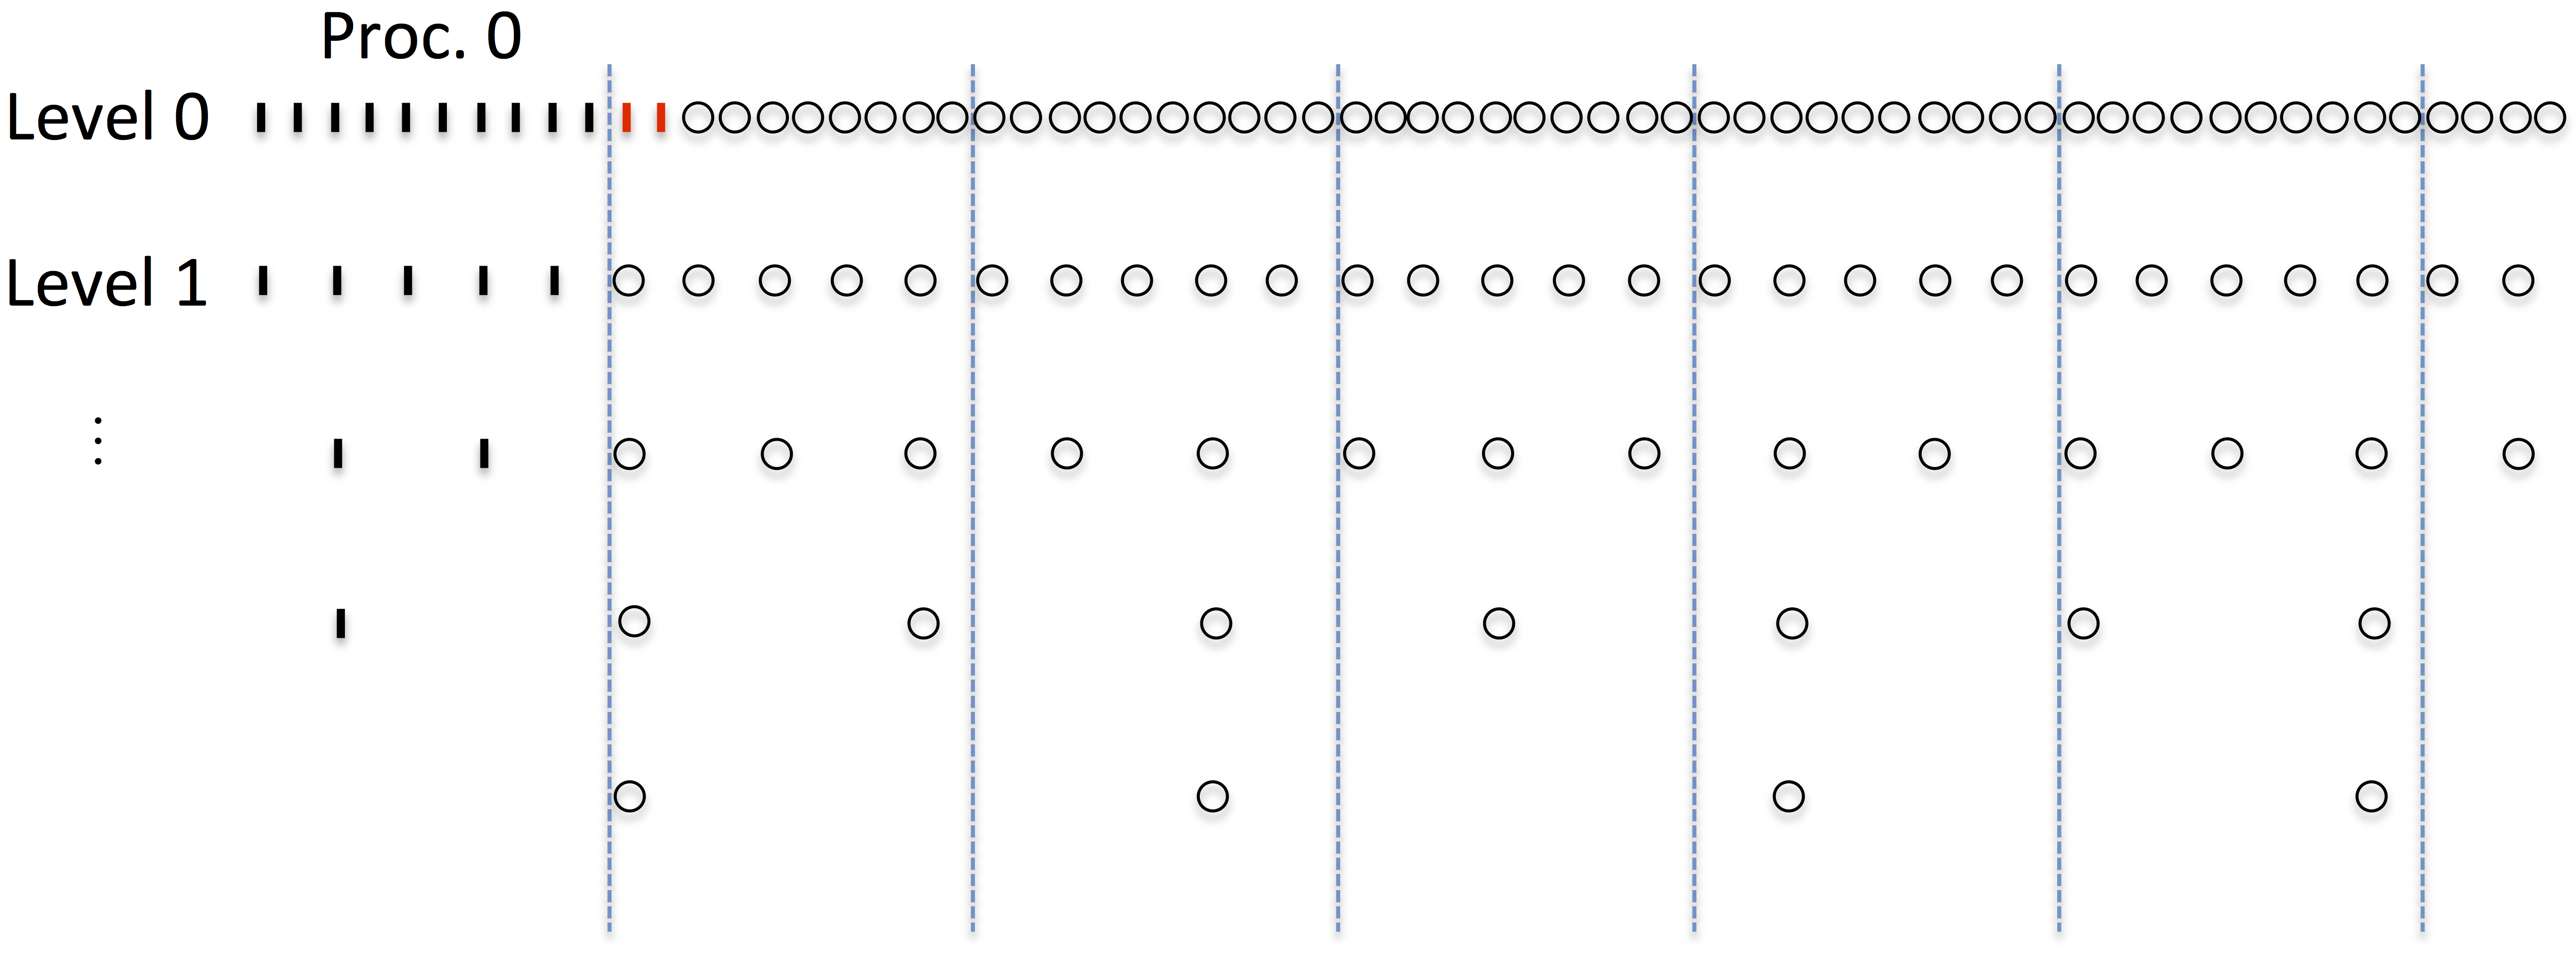
\includegraphics[width=\textwidth]{../figures/compGridCreation1D4}}
\only<3>{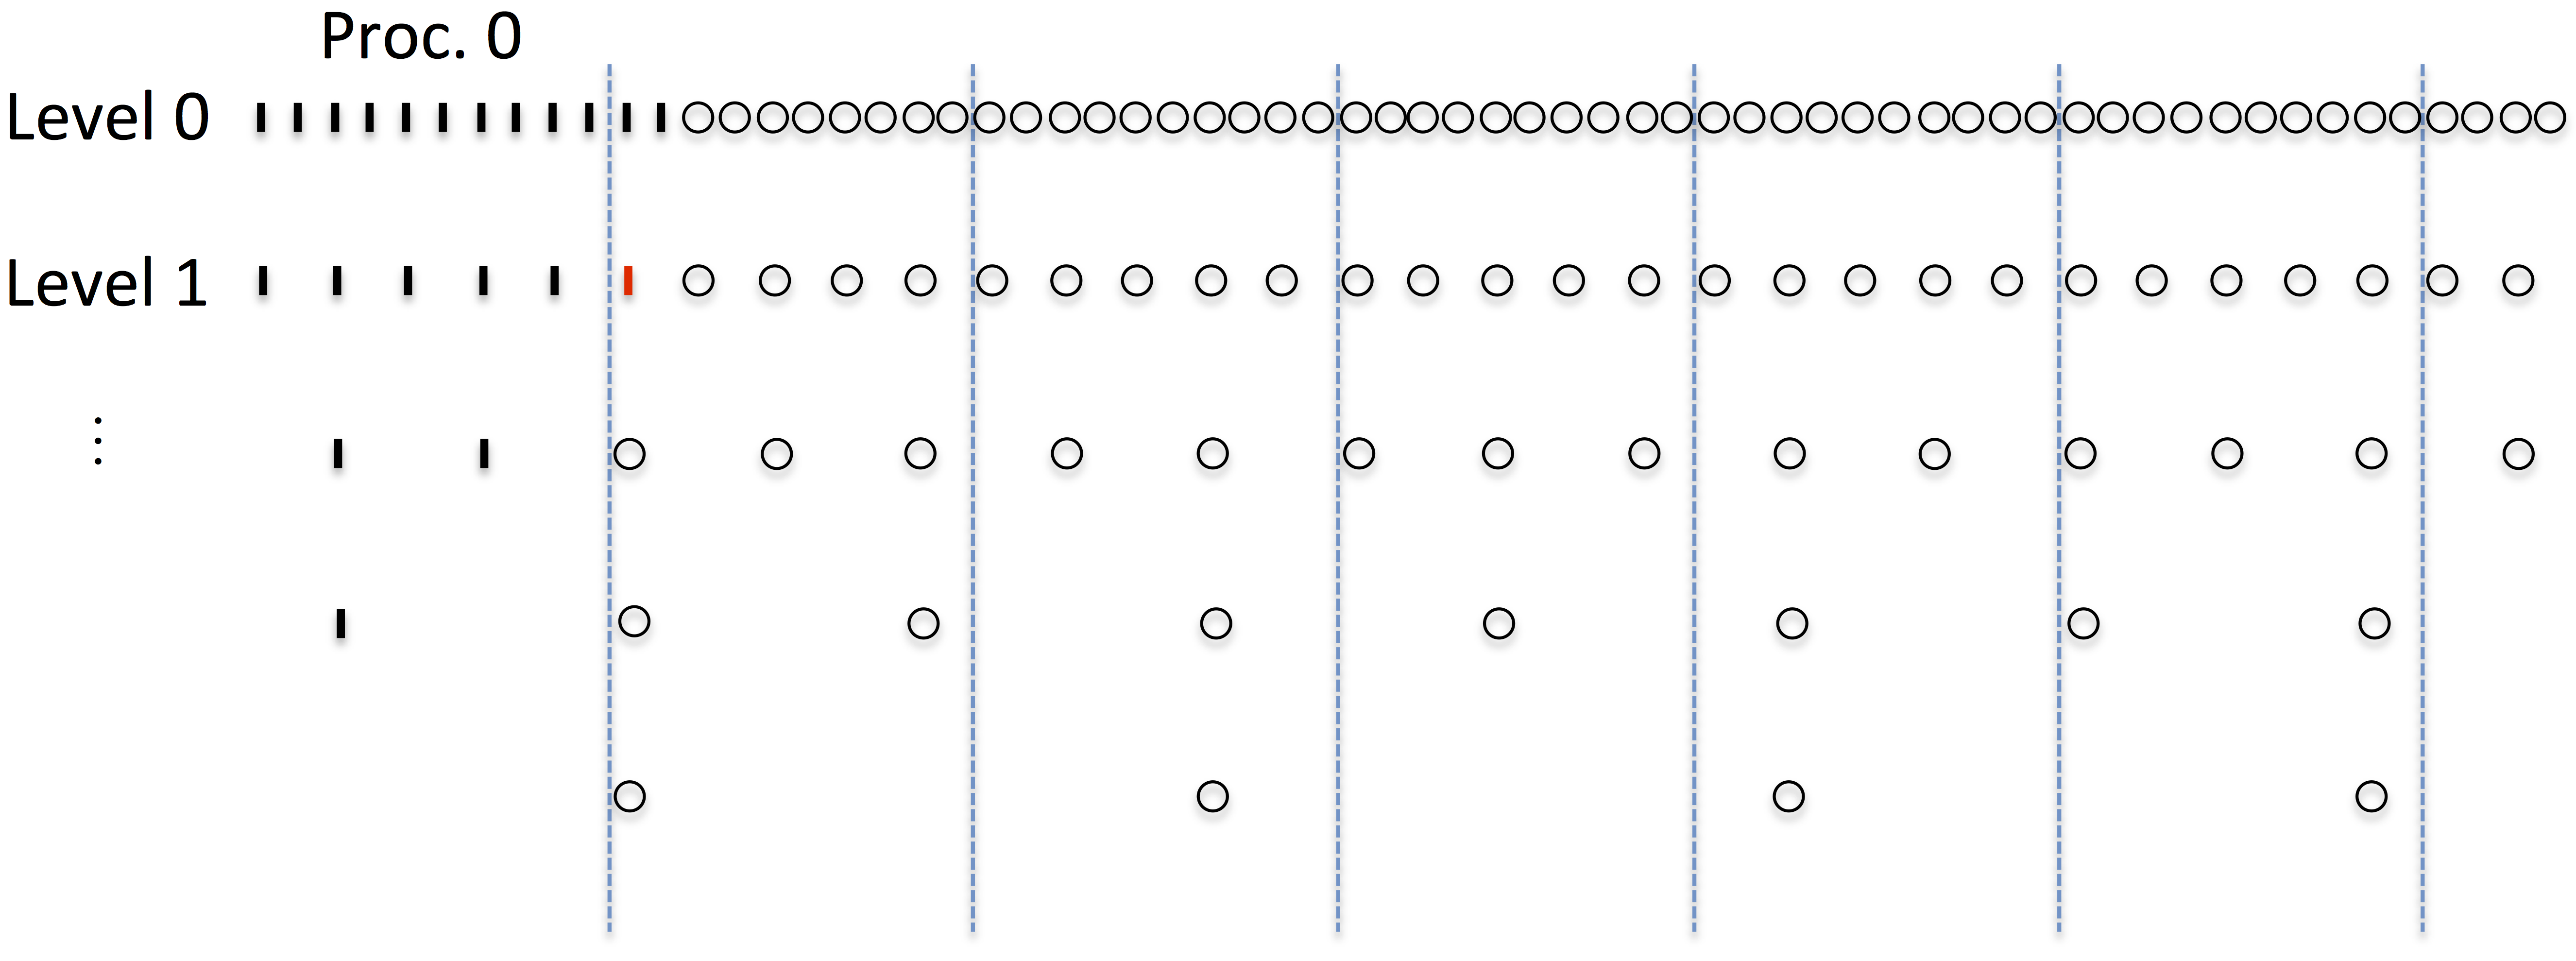
\includegraphics[width=\textwidth]{../figures/compGridCreation1D5}}
\only<4>{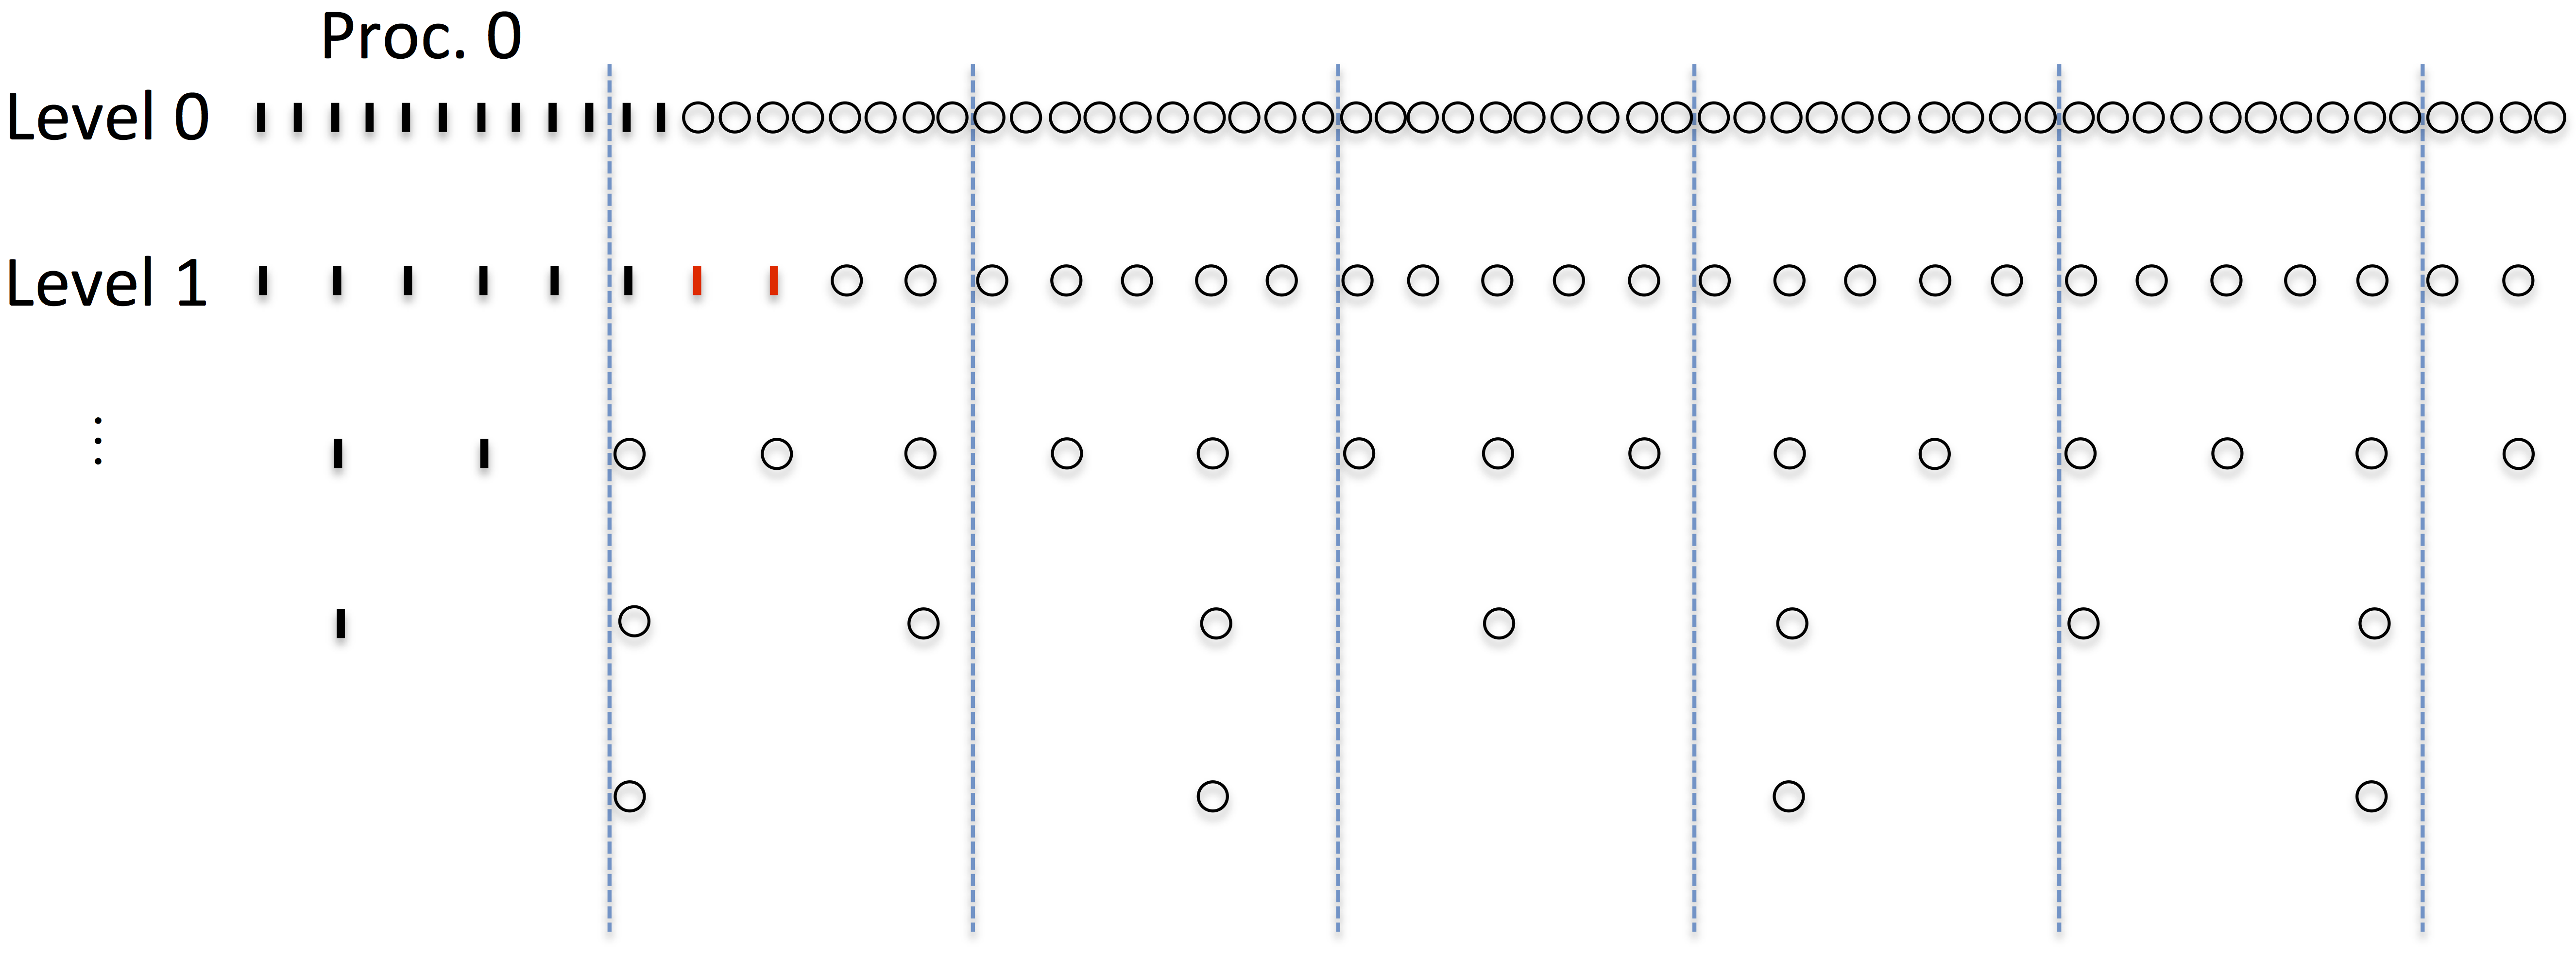
\includegraphics[width=\textwidth]{../figures/compGridCreation1D6}}
\only<5>{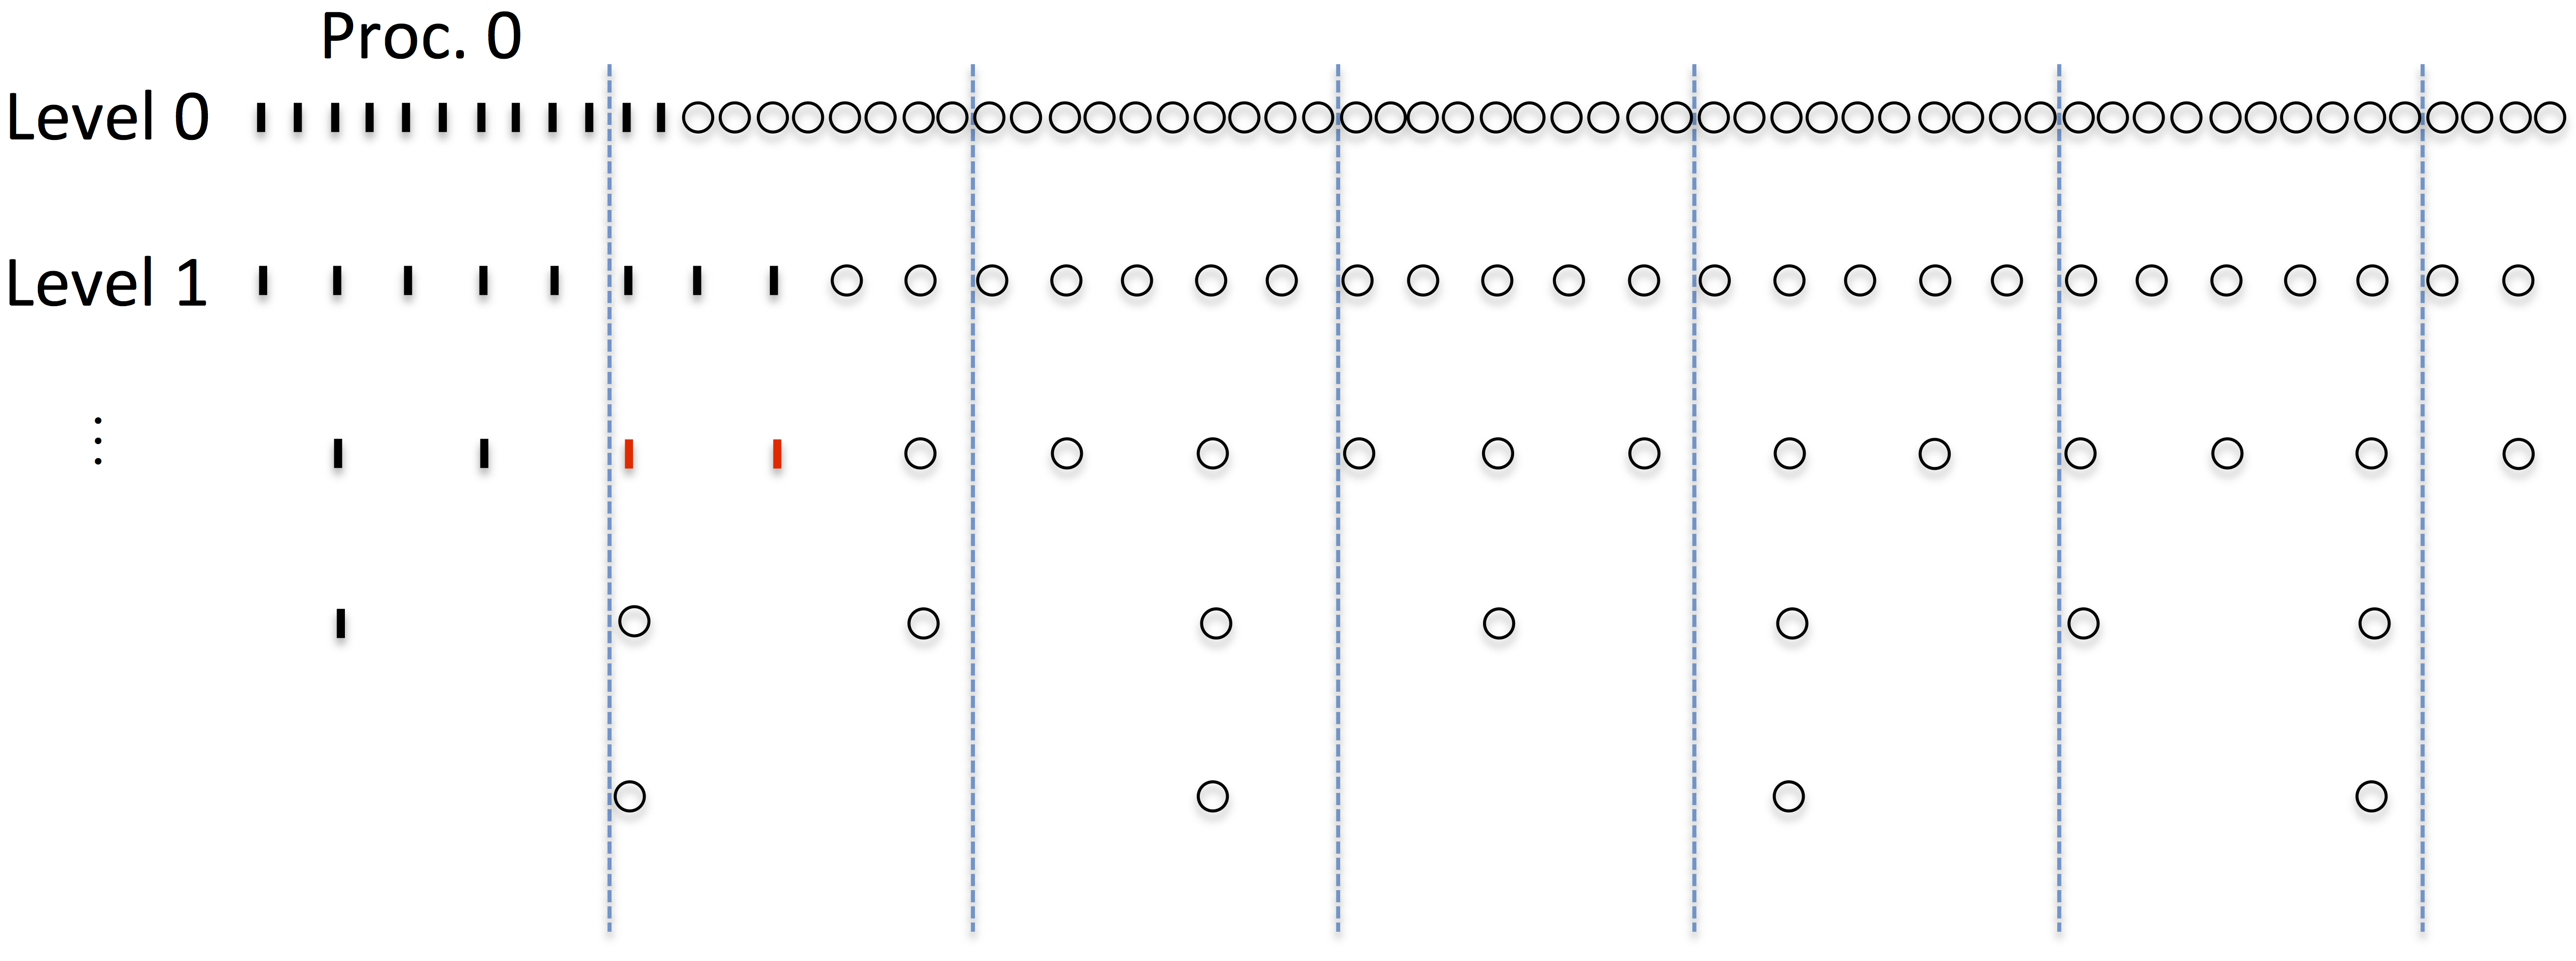
\includegraphics[width=\textwidth]{../figures/compGridCreation1D7}}
\only<6>{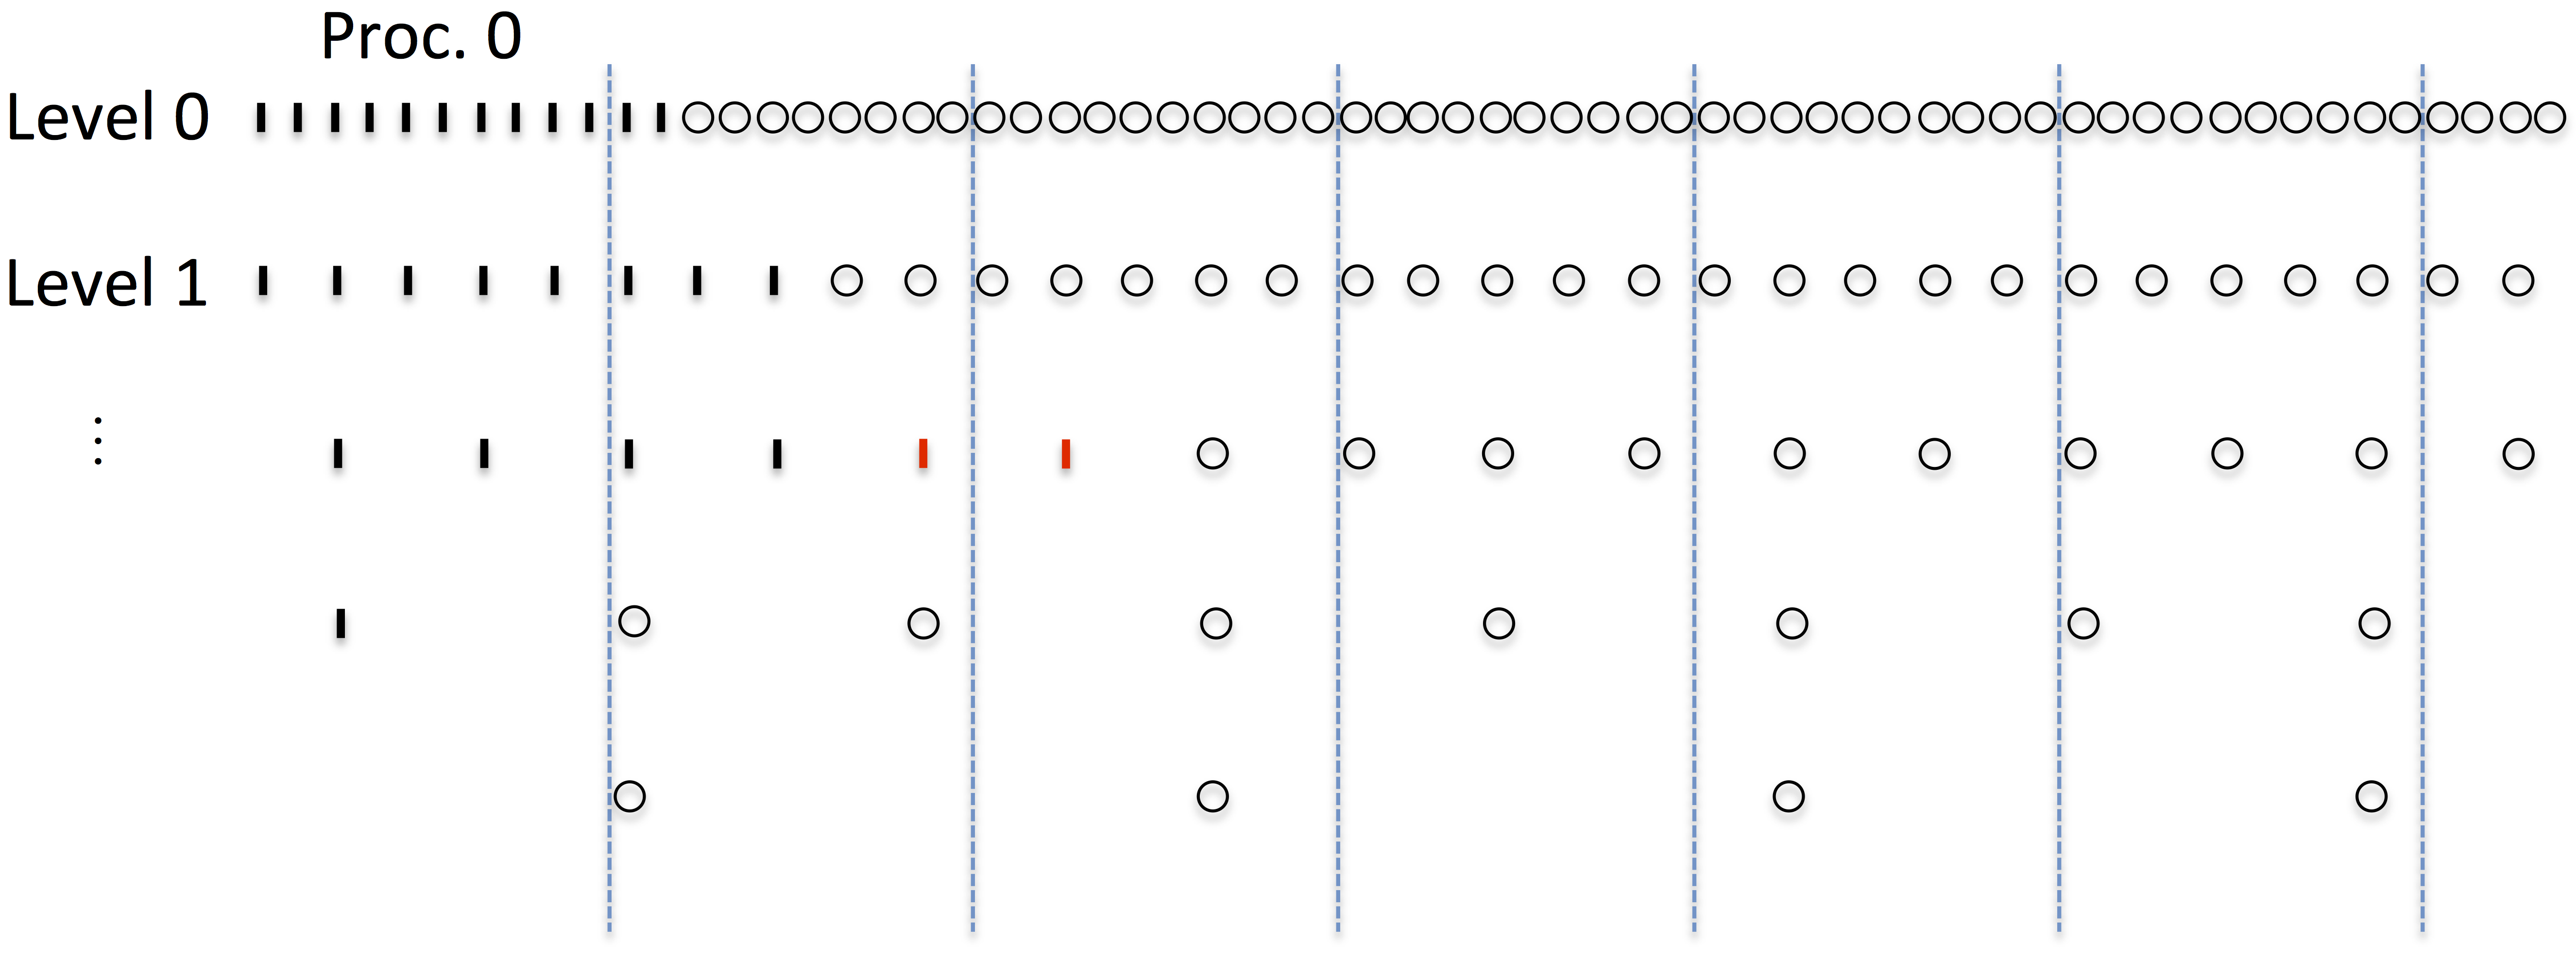
\includegraphics[width=\textwidth]{../figures/compGridCreation1D8}}
\only<7>{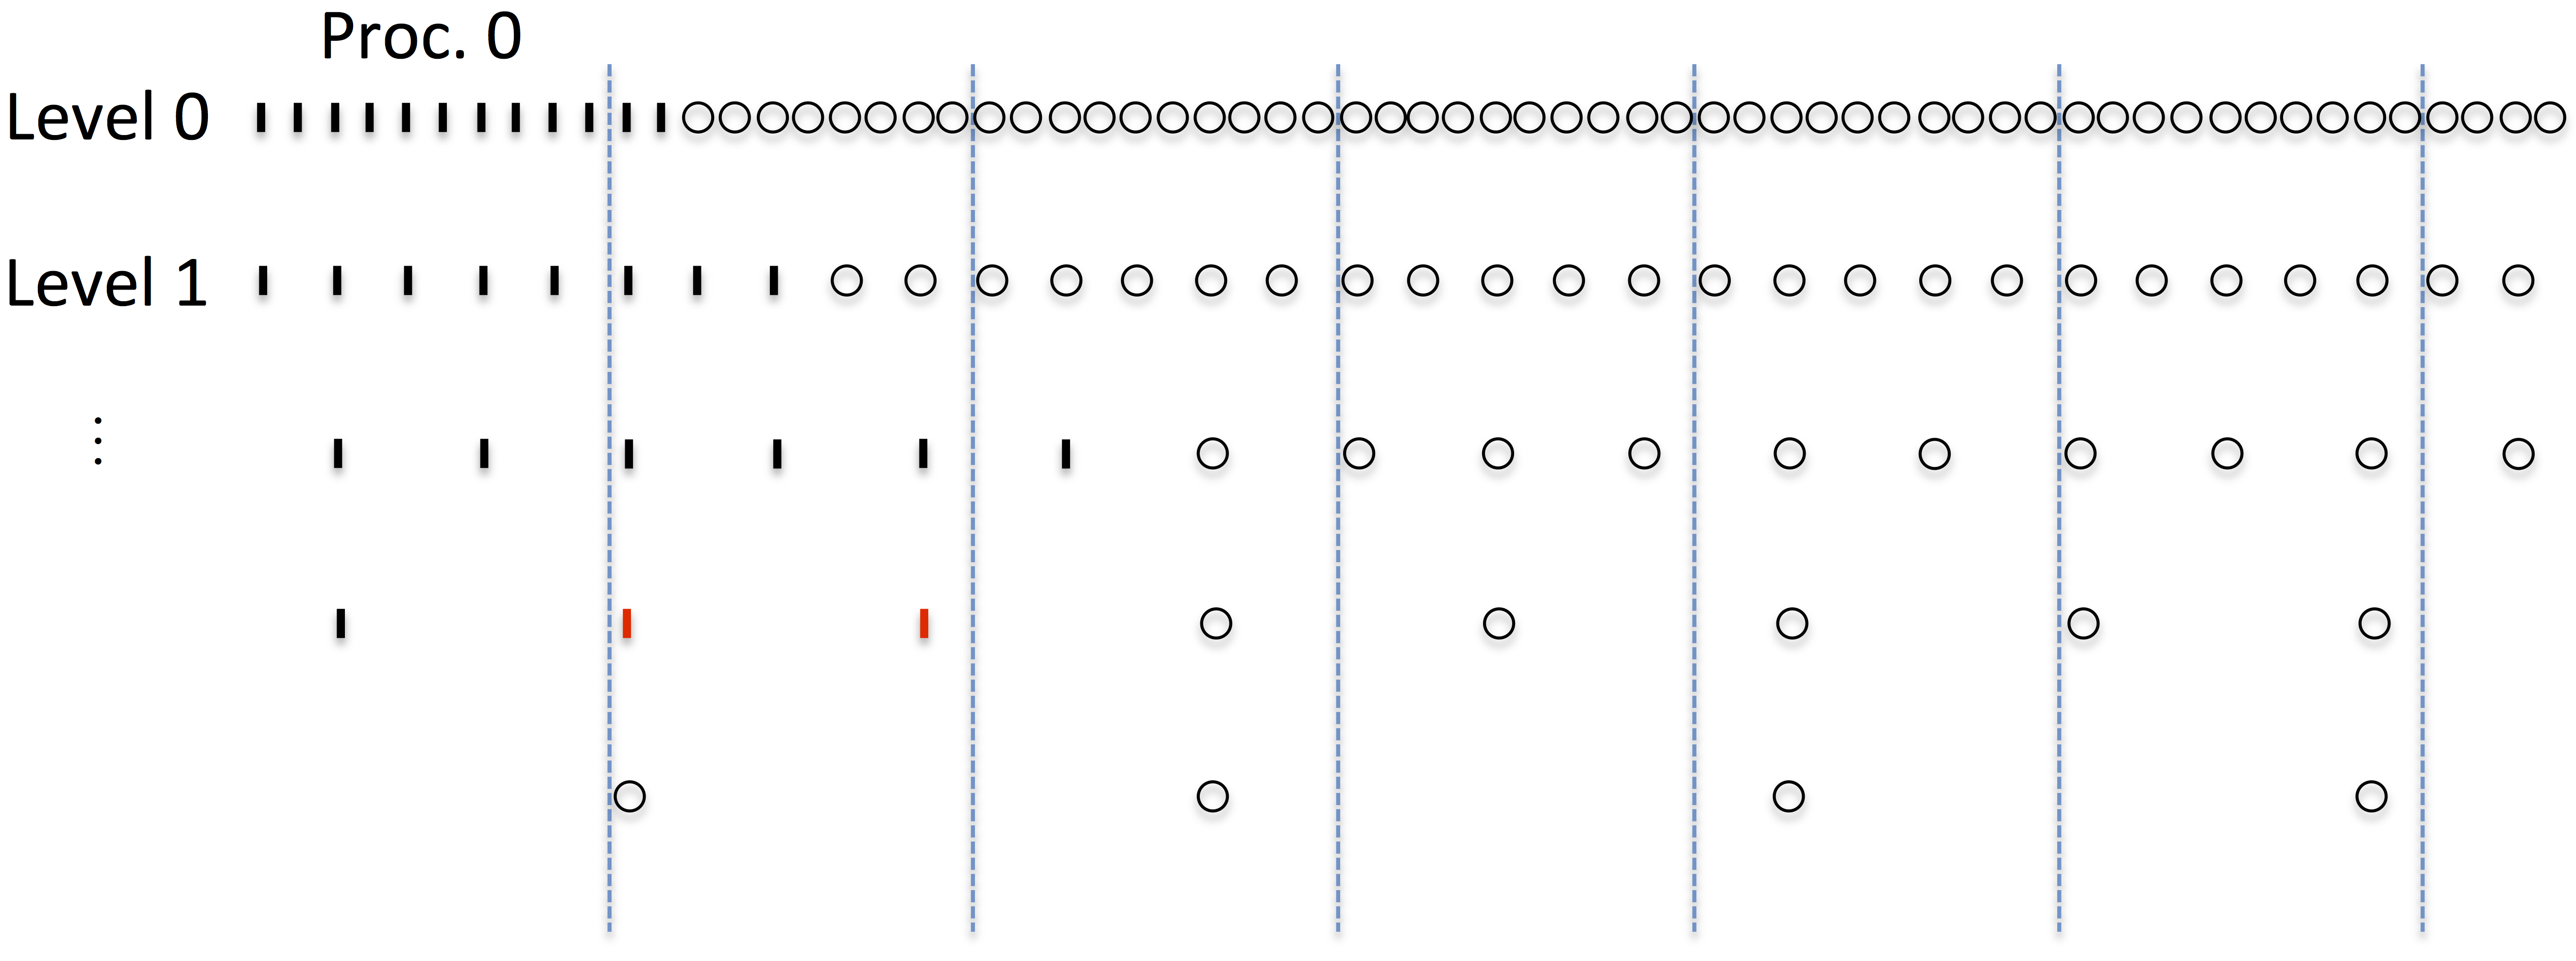
\includegraphics[width=\textwidth]{../figures/compGridCreation1D9}}
\only<8>{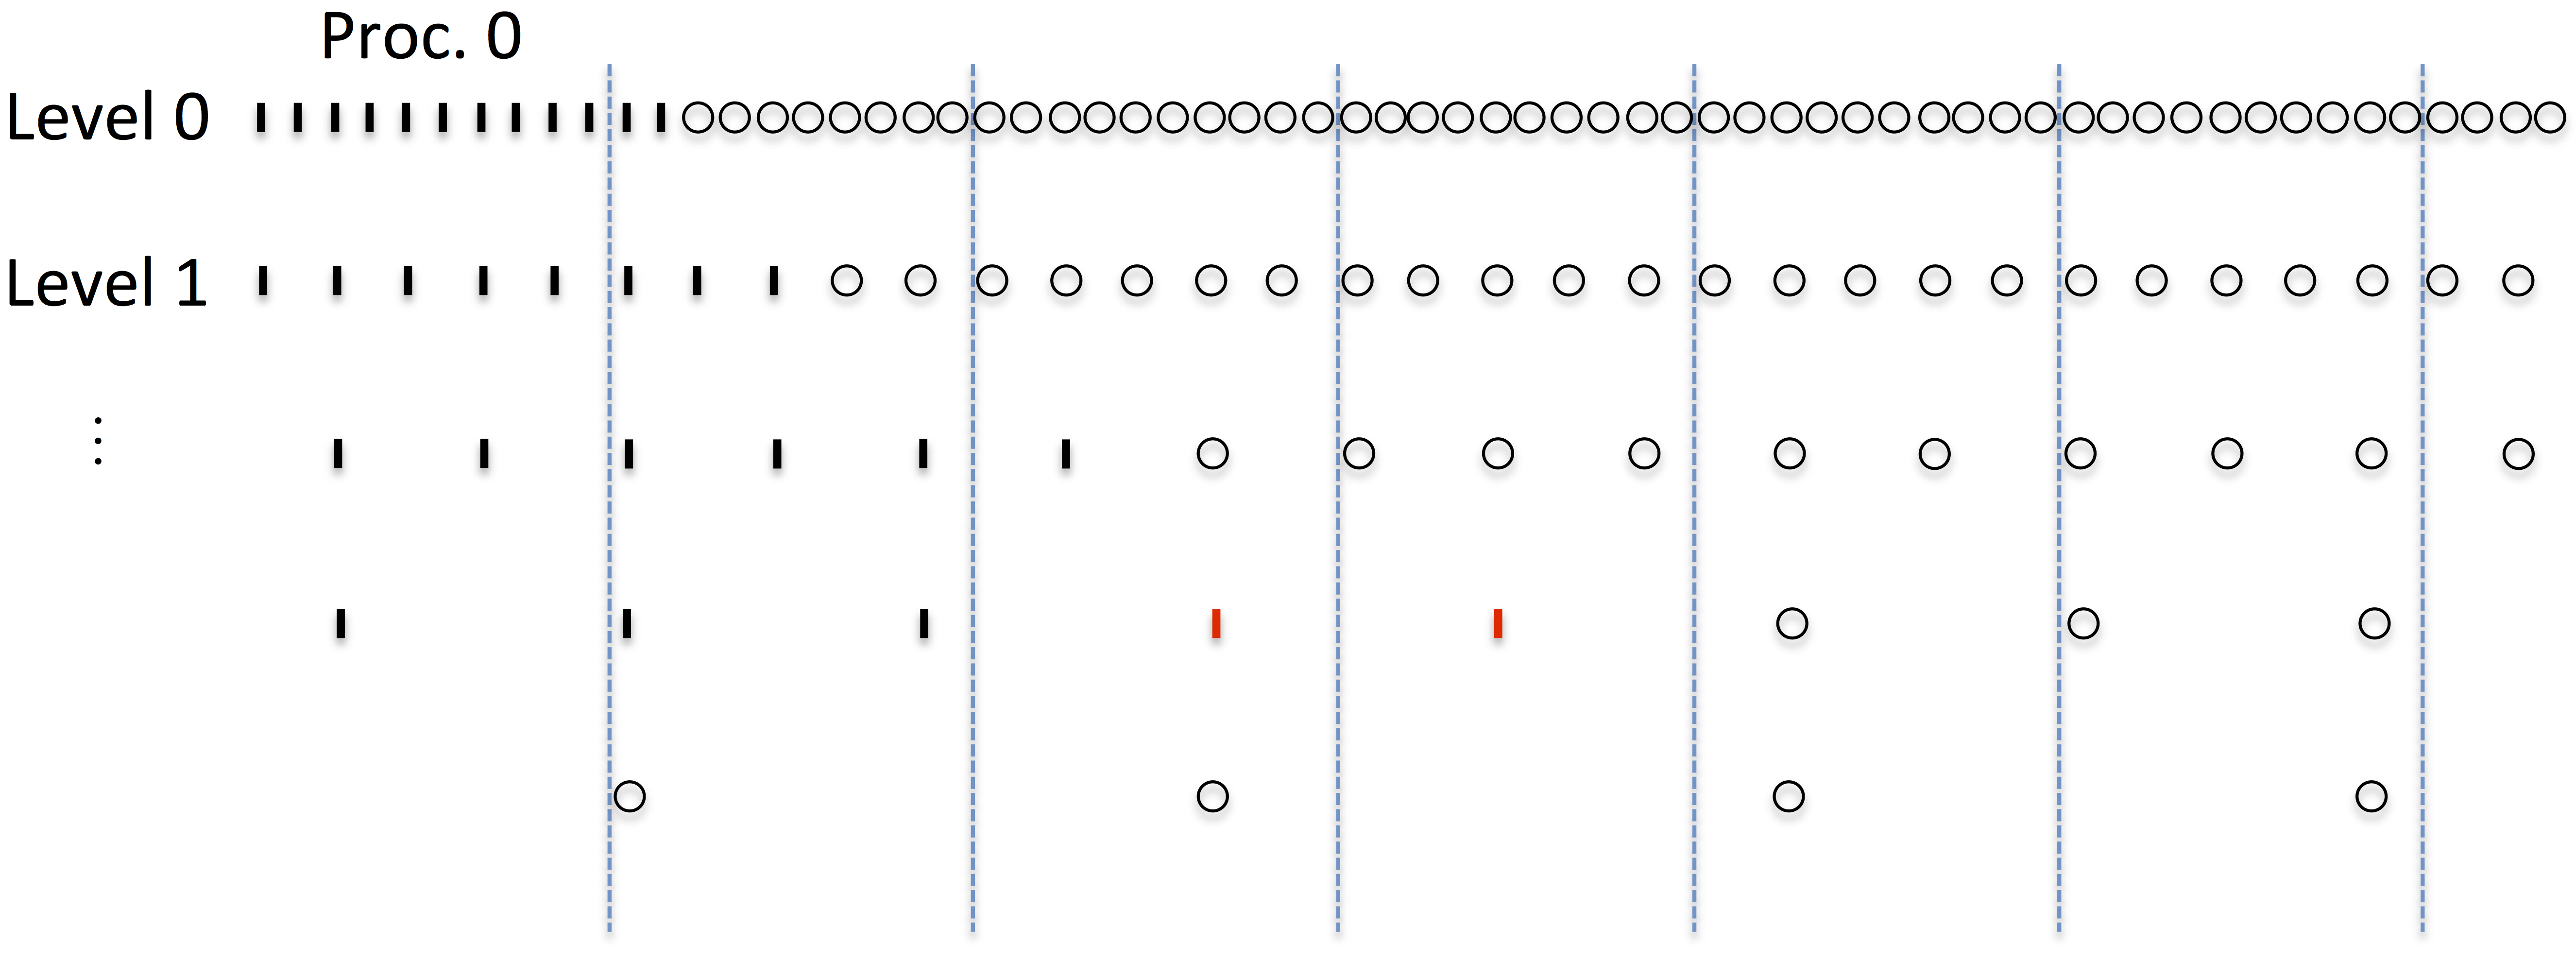
\includegraphics[width=\textwidth]{../figures/compGridCreation1D10}}
\only<9>{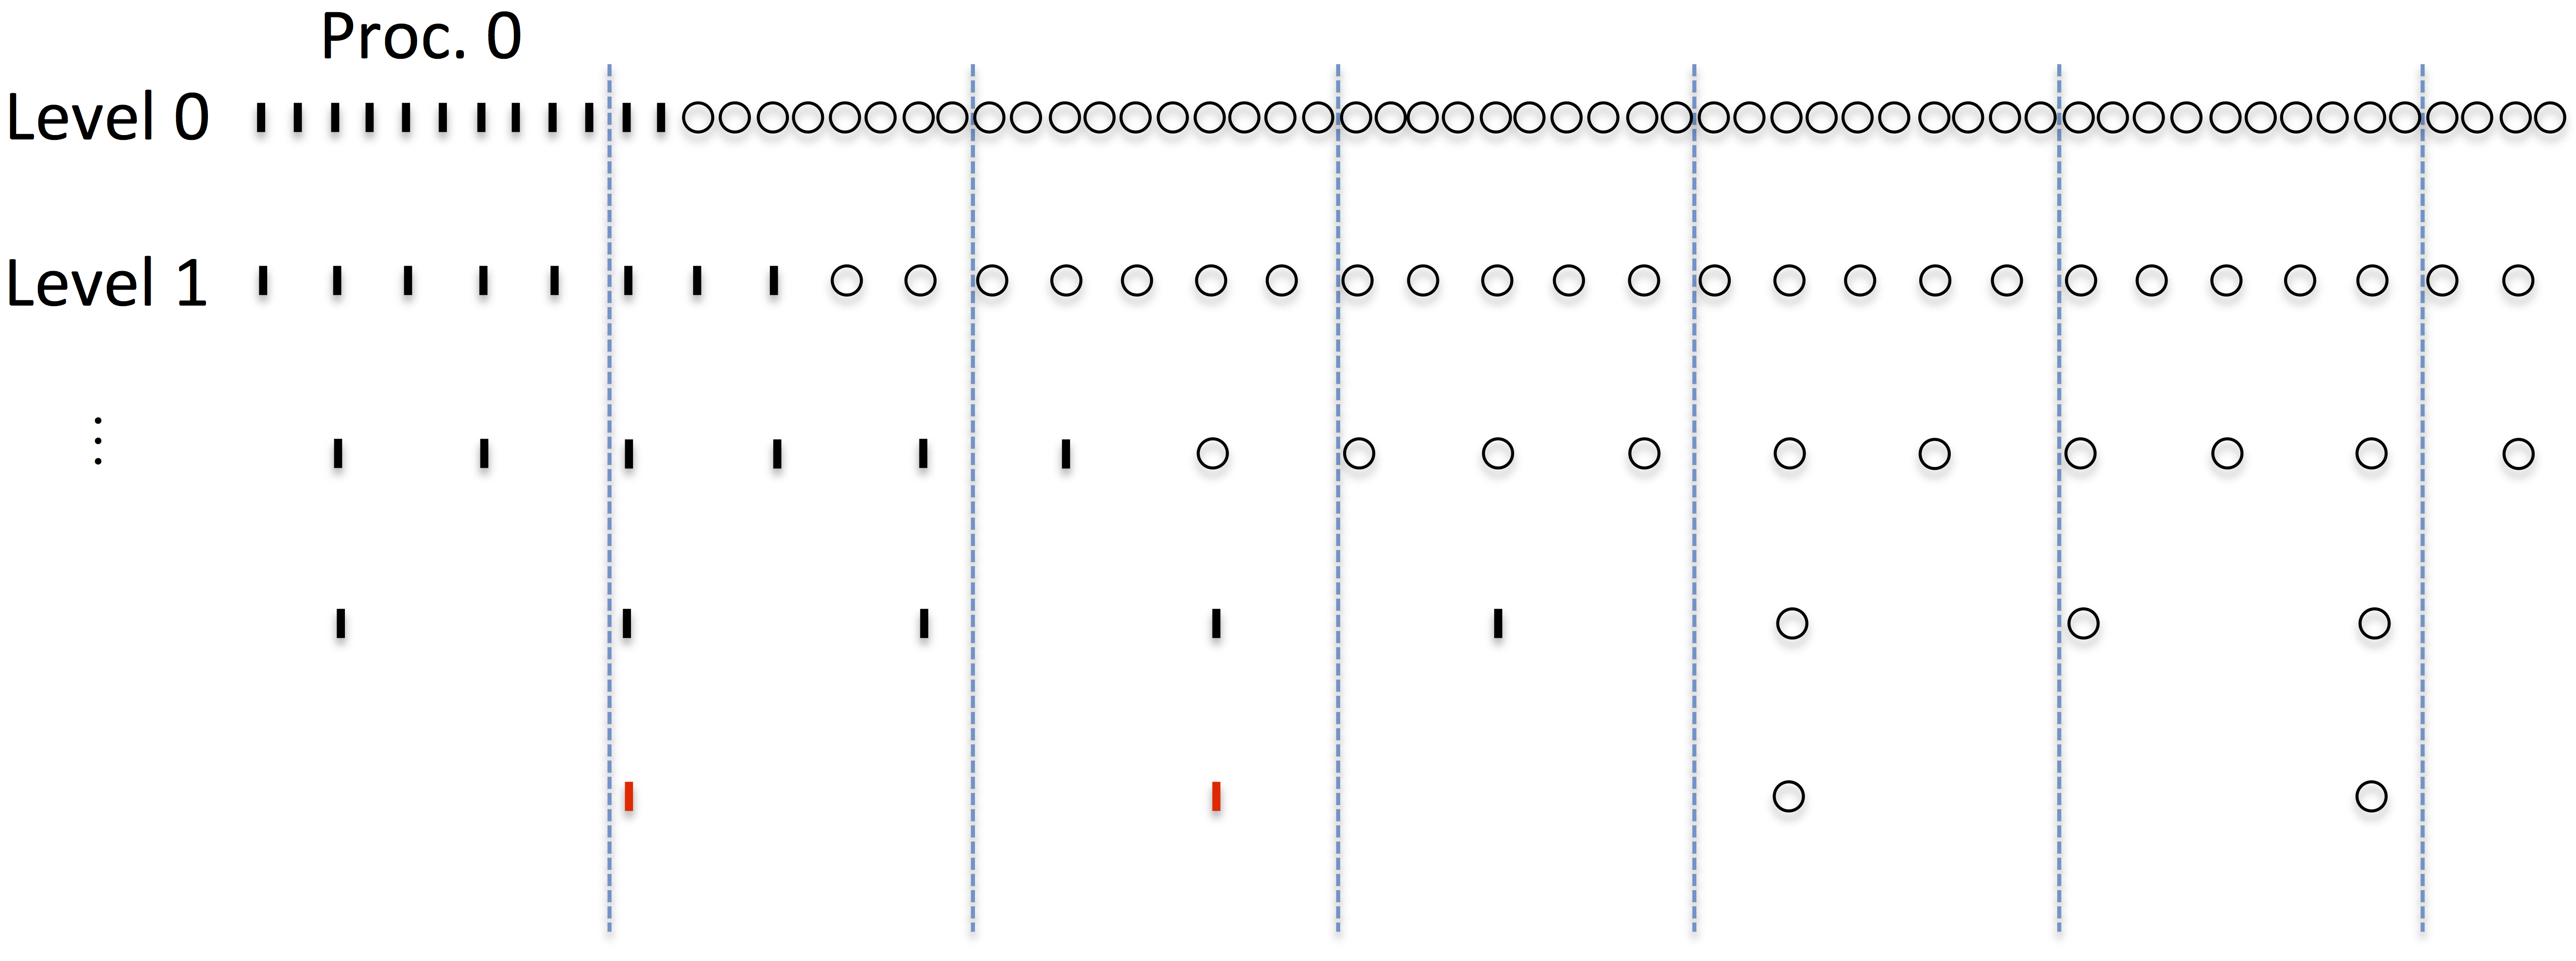
\includegraphics[width=\textwidth]{../figures/compGridCreation1D11}}
\only<10>{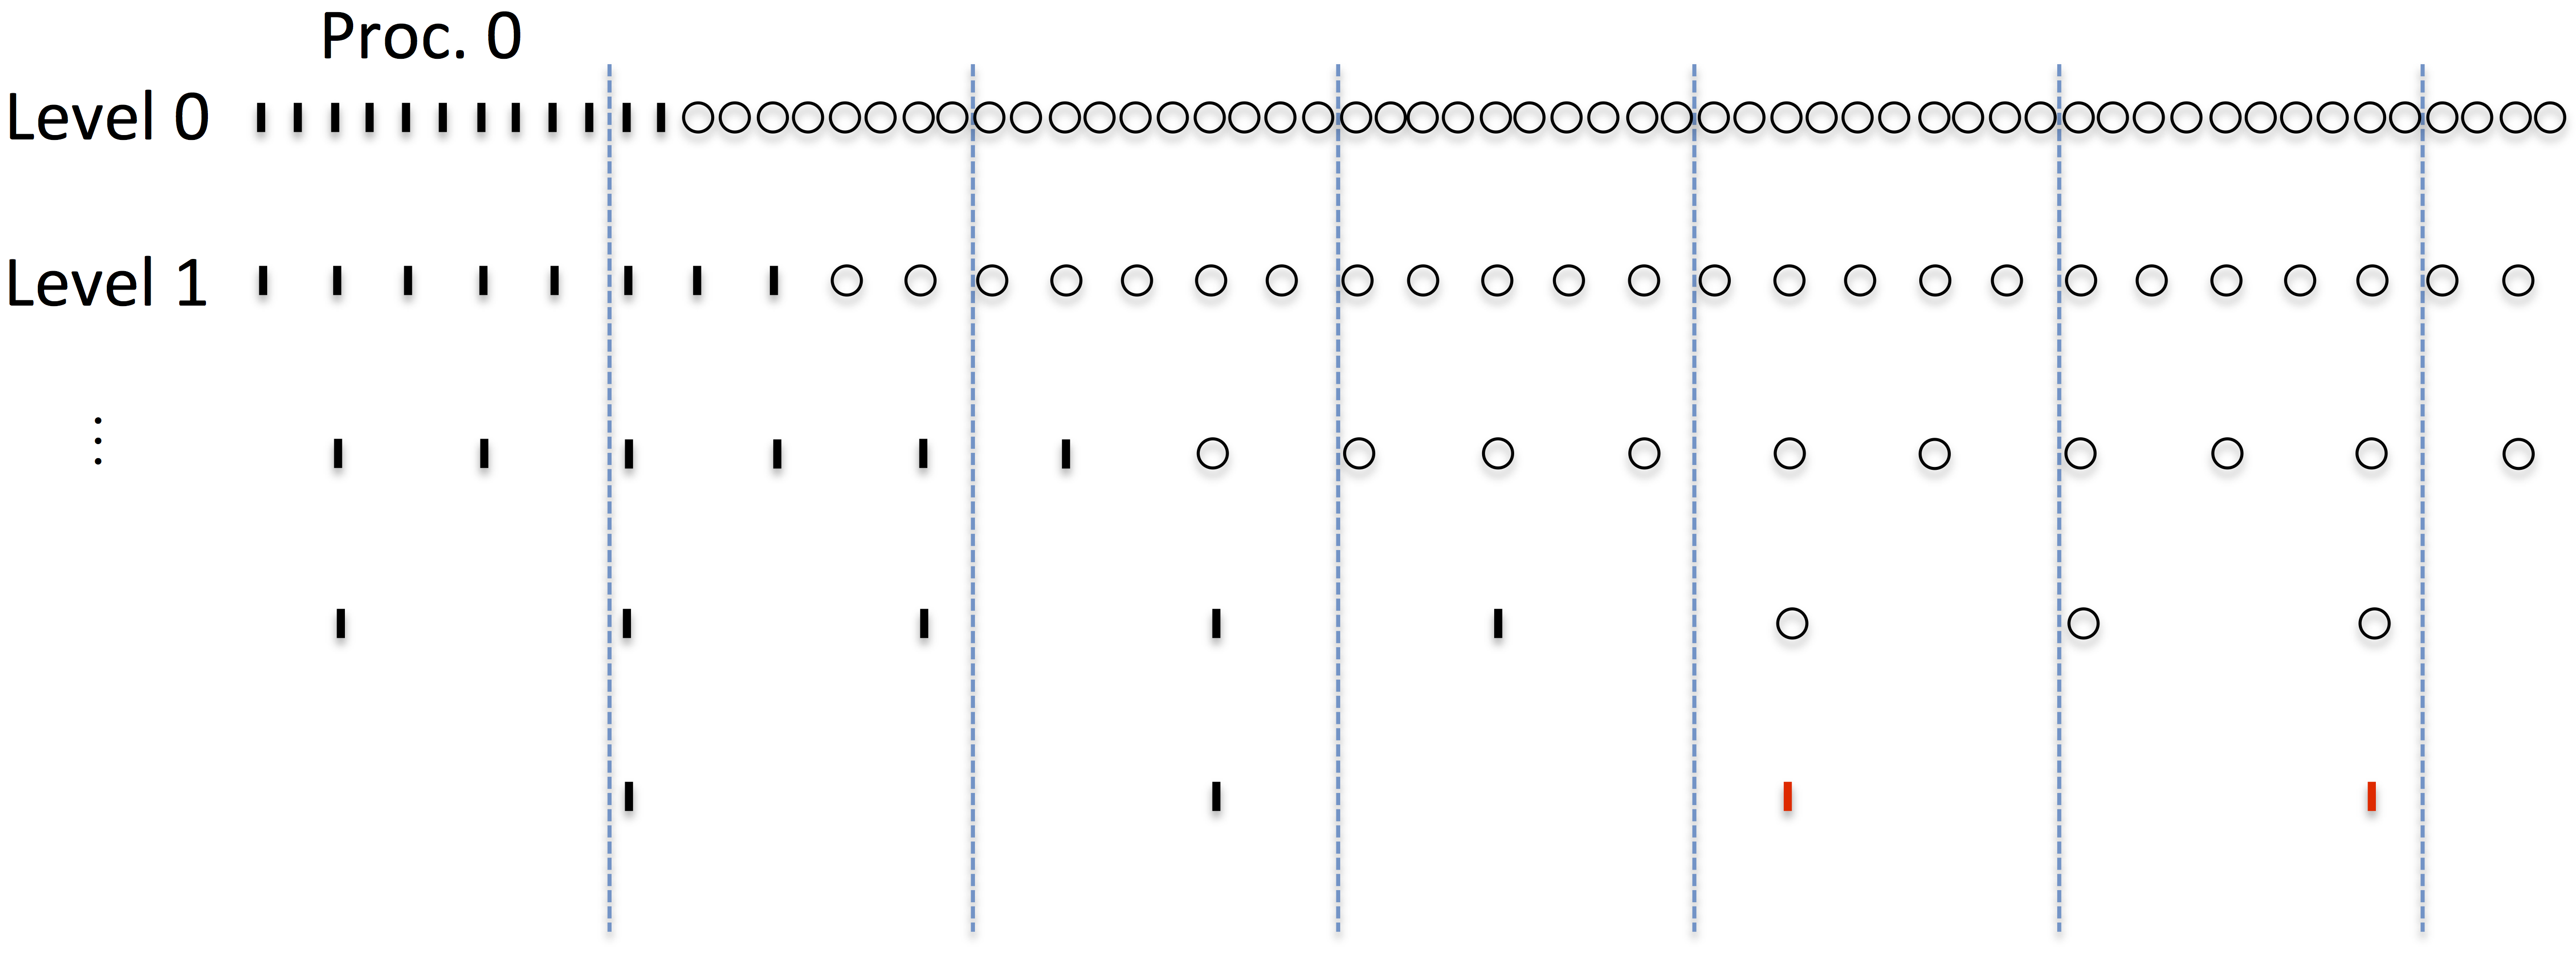
\includegraphics[width=\textwidth]{../figures/compGridCreation1D12}}
\only<11>{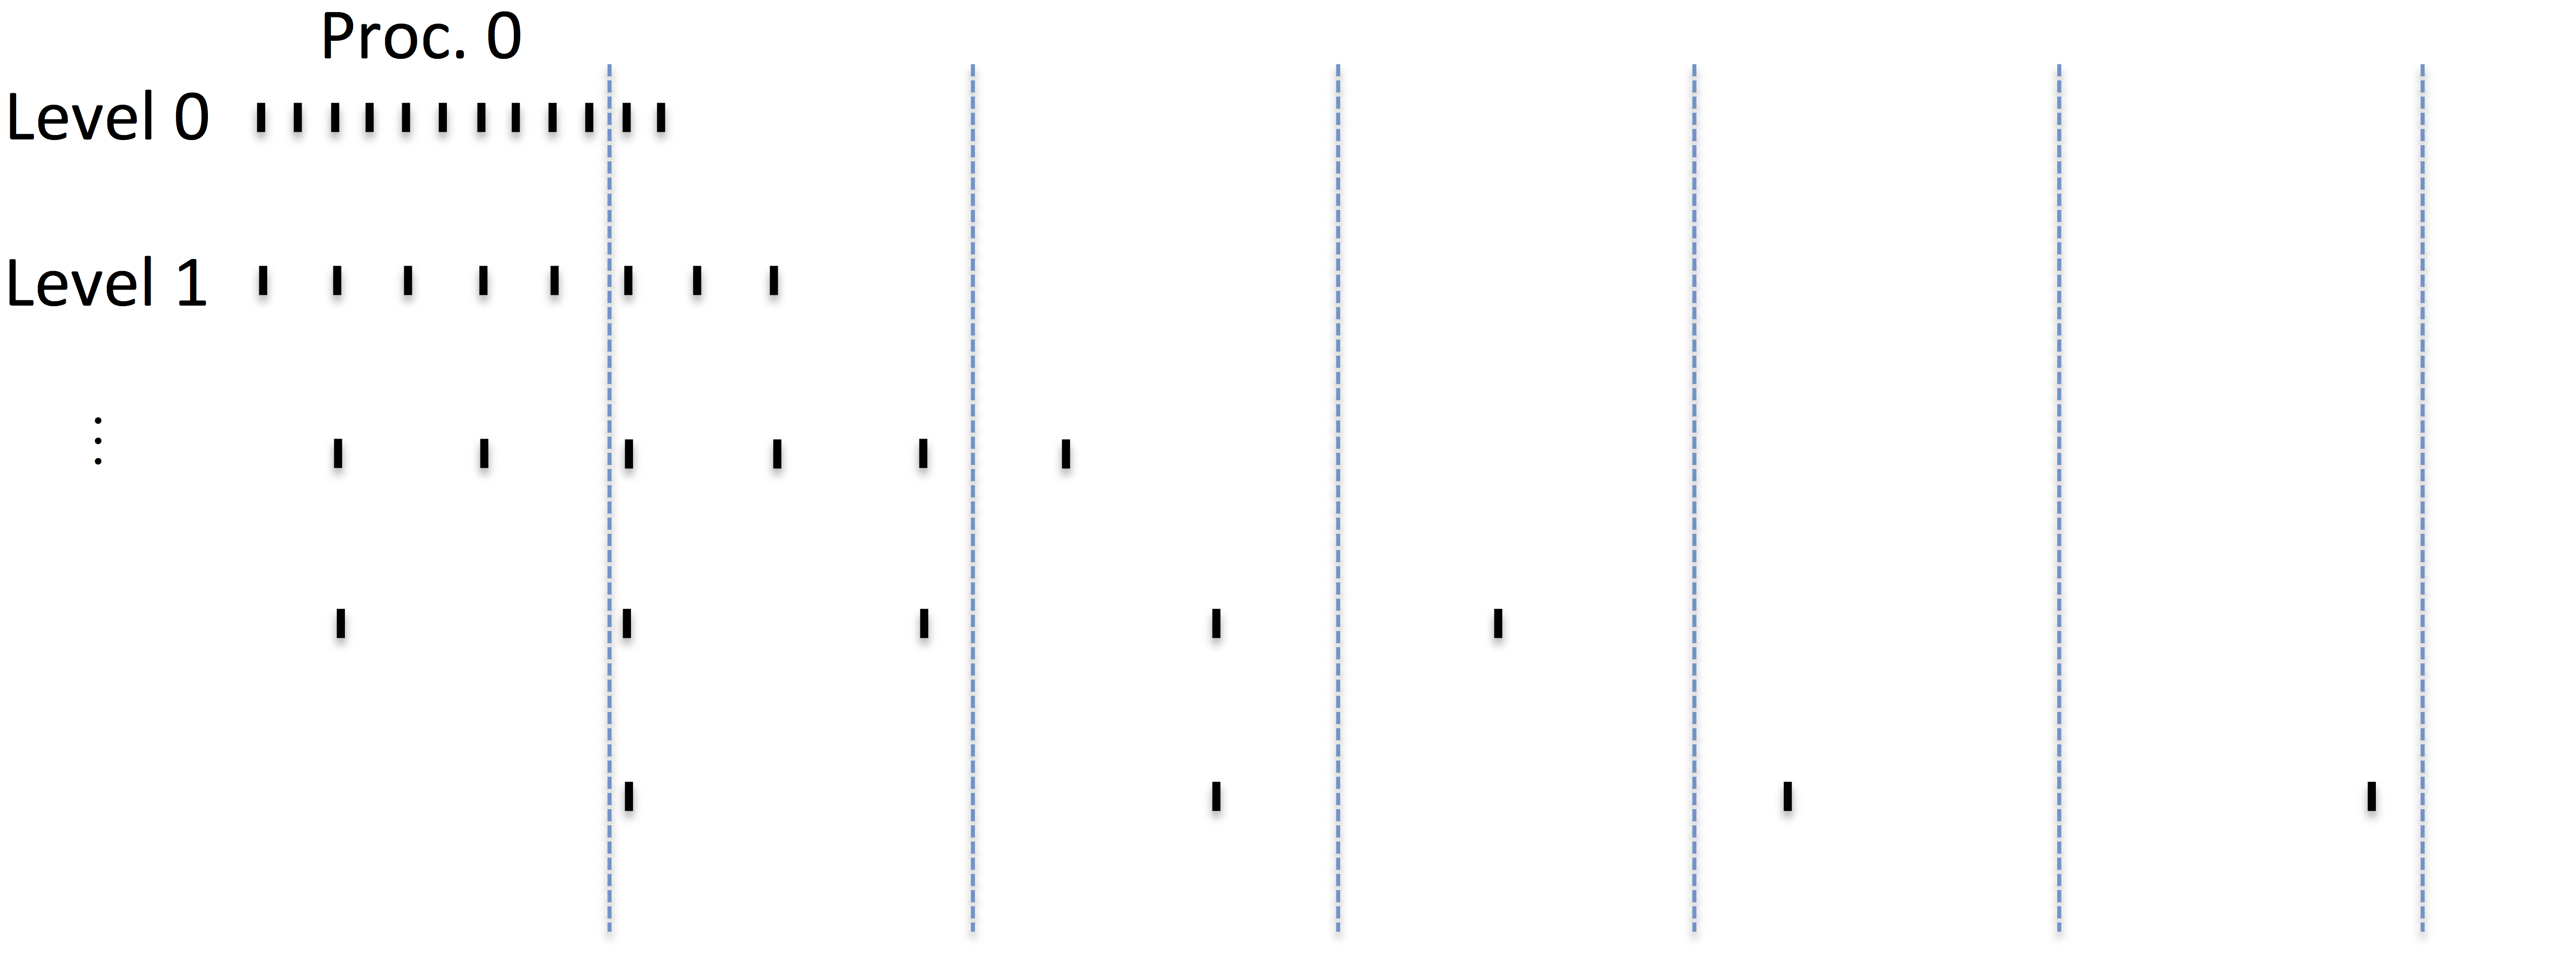
\includegraphics[width=\textwidth]{../figures/compGridCreation1D13}}
\end{frame}

% Slide
\begin{frame}{Algebraic multigrid domain decomposition (AMG-DD)}
\begin{block}{Features of the composite grid}
\begin{itemize}
\item Covers the entire computational domain
\item Cycling requires no communication 
\item Fine resolution in and near the processor subdomain
\item Goal: composite solution is accurate to the full solution over the processor subdomain
\end{itemize}
\end{block}

\end{frame}

% Slide
\begin{frame}{Algebraic multigrid domain decomposition (AMG-DD)}
\begin{block}{AMG-DD pseudo code}
\begin{itemize}
\item Setup:
\begin{itemize}
\item Generate AMG hierarchy
\item Form composite grids
\end{itemize}
\item Iterate:
\begin{itemize}
\item Update fine-grid residual and restrict to all levels (communication)
\item Each processor obtains updated residual at all composite grid points (communication)
\item Each processor cycles on the composite grid (no communication)
\item The global solution is updated by patching together processor subdomains (no communication)
\end{itemize}
\end{itemize}
\end{block}

\end{frame}

%% Slide
%\begin{frame}{Algebraic multigrid domain decomposition (AMG-DD)}
%\begin{block}{Brief details: residual communication}
%\begin{itemize}
%\item Proceeds from coarse to fine level
%\item Communication patterns based on padding
%\end{itemize}
%\end{block}
%
%\centering
%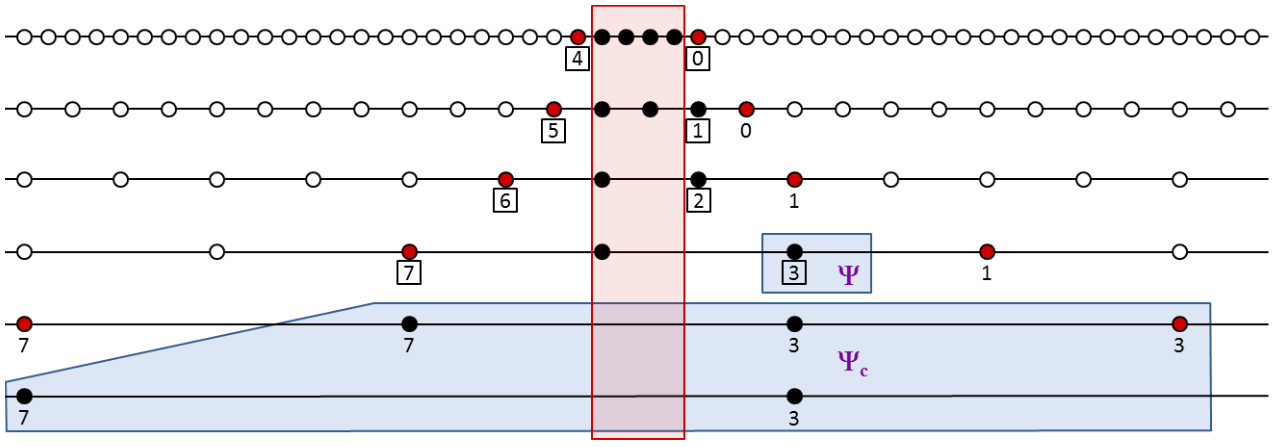
\includegraphics[width=0.7\textwidth]{../figures/resComm}
%
%\hspace{0.5 cm}
%
%\tiny{Figure taken from \emph{Algebraic multigrid domain and range decomposition (AMG-DD/AMG-RD)} by Bank, Falgout, Jones, Manteuffel, McCormick, and Ruge.}
%
%\end{frame}

% Slide
\begin{frame}{Algebraic multigrid domain decomposition (AMG-DD)}
\begin{block}{Brief details: residual communication}
\begin{itemize}
\item Communication on each level moving from coarse to fine
\item Communication stencils are based on padding
\item With padding 1, same communication pattern as operator matrix-vector multiplies on each level 
\end{itemize}
\end{block}

\end{frame}

% Slide
\begin{frame}{Algebraic multigrid domain decomposition (AMG-DD)}
\begin{block}{Brief details: composite-grid solve}
\begin{itemize}
\item Fast adaptive composite (FAC) cycle
\item Action is equivalent to global cycle with suppressed relaxation
\end{itemize}
\end{block}

\centering
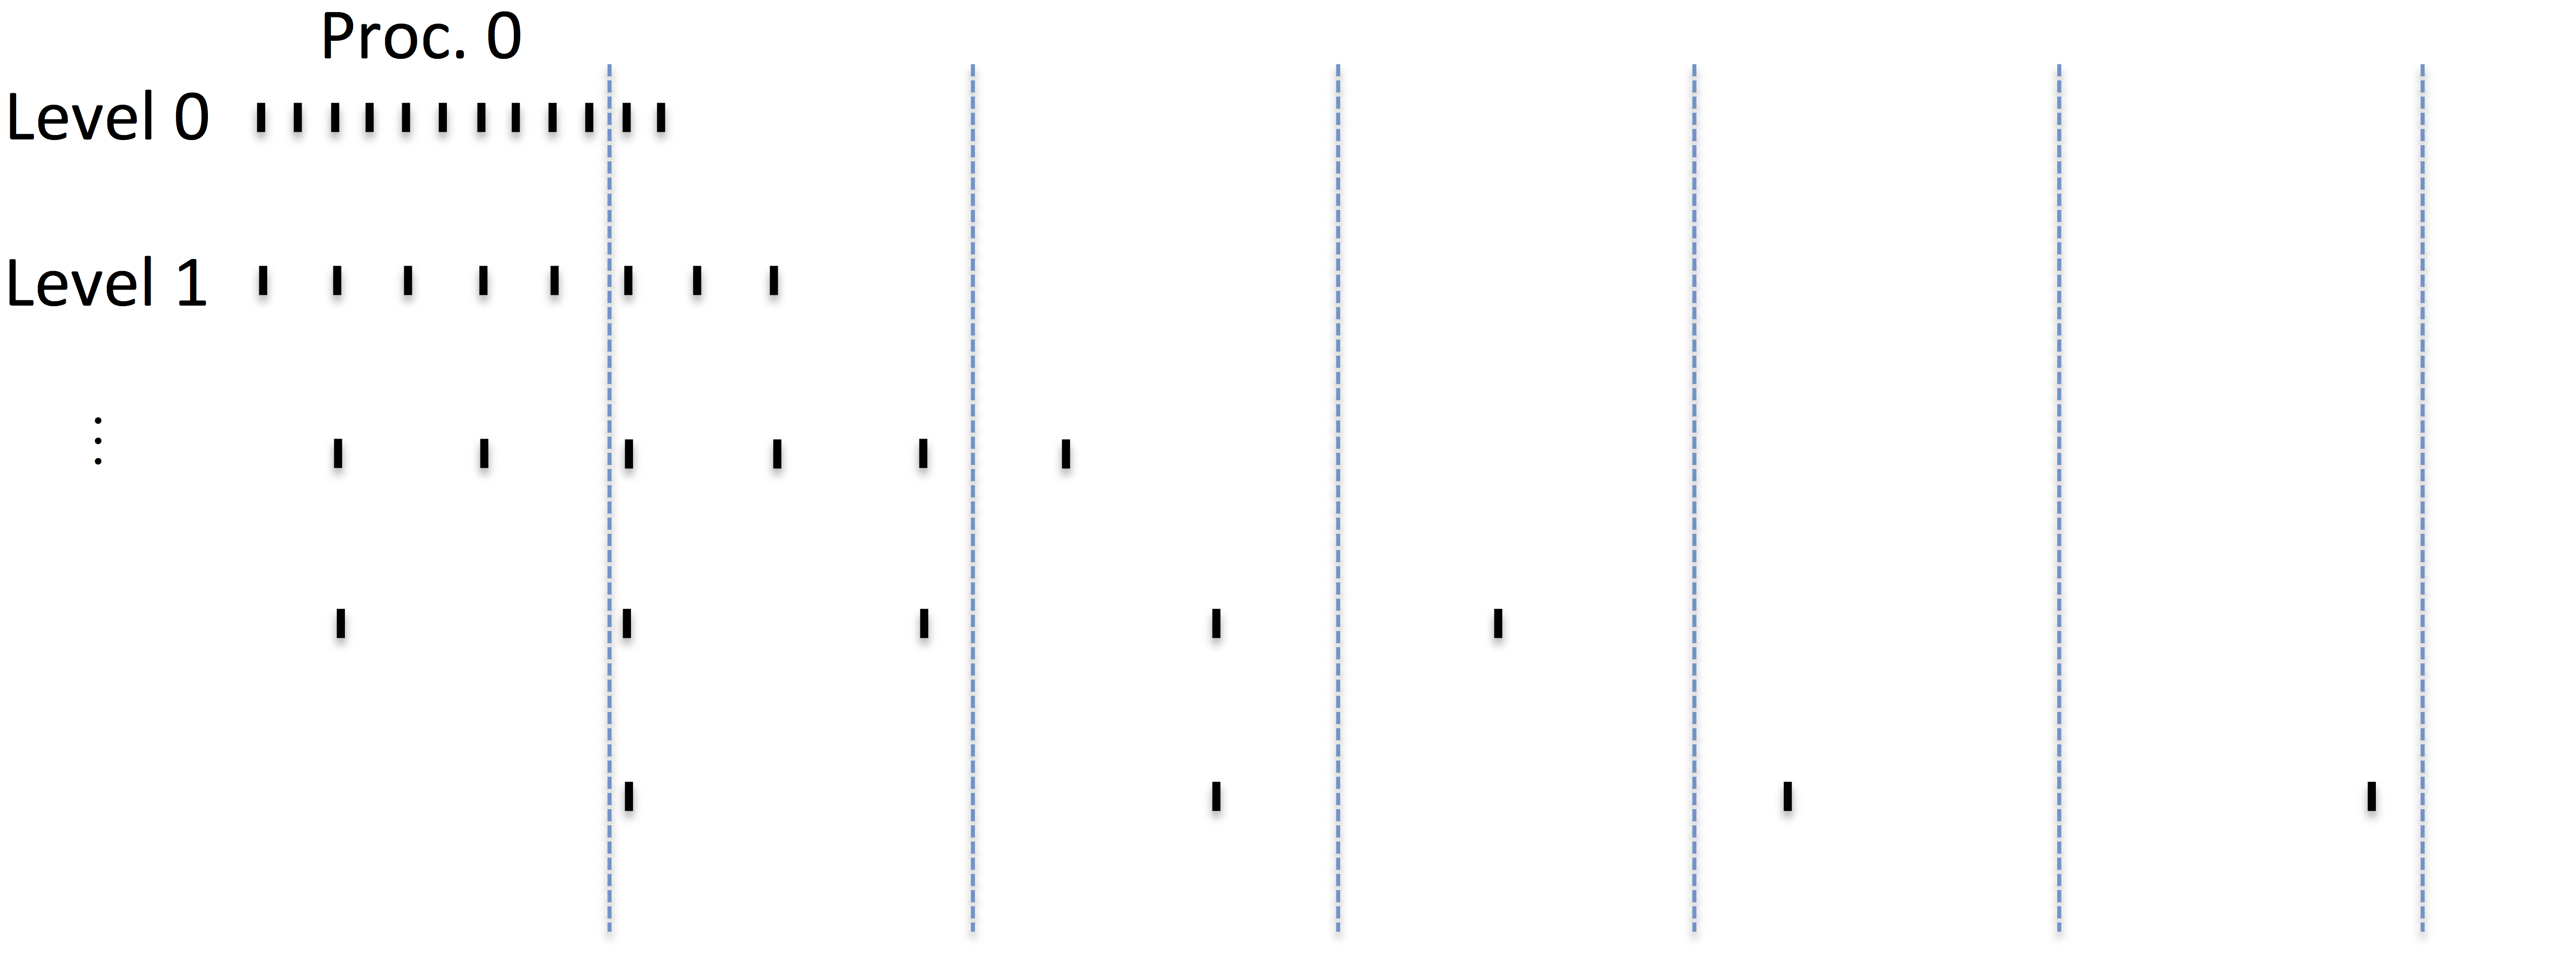
\includegraphics[width=\textwidth]{../figures/compGridCreation1D13}

\end{frame}

% Slide
\begin{frame}{Algebraic multigrid domain decomposition (AMG-DD)}
\begin{block}{Test problems}

\begin{align*}
-\nabla \cdot K \nabla u &= \mathbf{1}\,, \hspace{1 cm} \Omega \\
u &= 0\,, \hspace{1 cm} \partial \Omega
\end{align*}

\begin{itemize}
\item 3D Poisson: $K = I$ and $\Omega$ is the unit cube
\item 2D rotated anisotropic diffusion: $\Omega$ is the unit square, $K = Q^TDQ$
\end{itemize}

\begin{align*}
Q &= \begin{bmatrix}
\cos(\theta) & \sin(\theta) \\
-\sin(\theta) & \cos(\theta)
\end{bmatrix}
&
D &= \begin{bmatrix}
1 & 0\\
0 & \epsilon
\end{bmatrix}
\end{align*}
with $\theta=\pi/8$ and $\epsilon=0.001$
\end{block}


\end{frame}

% Slide
\begin{frame}{Algebraic multigrid domain decomposition (AMG-DD)}
\begin{block}{Parameters}
\begin{itemize}
\item Implementation on top of BoomerAMG in hypre
\item AMG best-practices parameters:
\begin{itemize}
   \item Coarsening: HMIS
   \item Interpolation: extended + i
\end{itemize}
\item AMG-DD parameters:
\begin{itemize}
   \item Padding
   \item Number of FAC cycles
\end{itemize}
\item Problem setup:
\begin{itemize}
   \item 256 processors
   \item 12,000 or 18,000 degrees of freedom per processor
\end{itemize}
\end{itemize}
\end{block}

\end{frame}

% Slide
\begin{frame}{Algebraic multigrid domain decomposition (AMG-DD)}
\begin{block}{Padding}
Larger padding yields:
\begin{itemize}
   \item Better accuracy to the global problem
   \item Larger composite grids
   \item More communication and computation
\end{itemize}
\end{block}

\centering
\vspace{0.5 cm}
% \includegraphics[height=0.3\textwidth]{../figures/resConvPadProb0}
% \includegraphics[height=0.3\textwidth]{../figures/resConvPadProb2}

\end{frame}

%% Slide
%\begin{frame}{Algebraic multigrid domain decomposition (AMG-DD)}
%\begin{block}{Padding}
%Larger padding yields:
%\begin{itemize}
%   \item Better accuracy to the global problem
%   \item Larger composite grids
%   \item More communication and computation
%\end{itemize}
%\end{block}
%
%\centering
%\vspace{0.5 cm}
%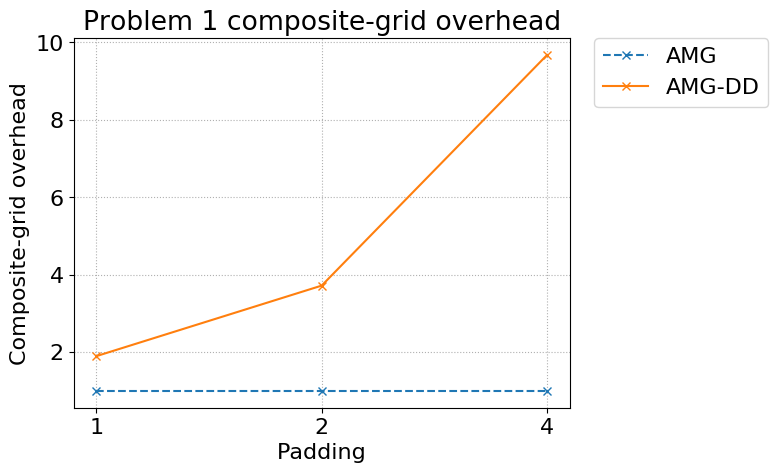
\includegraphics[height=0.3\textwidth]{../figures/gridSizePadProb0}
%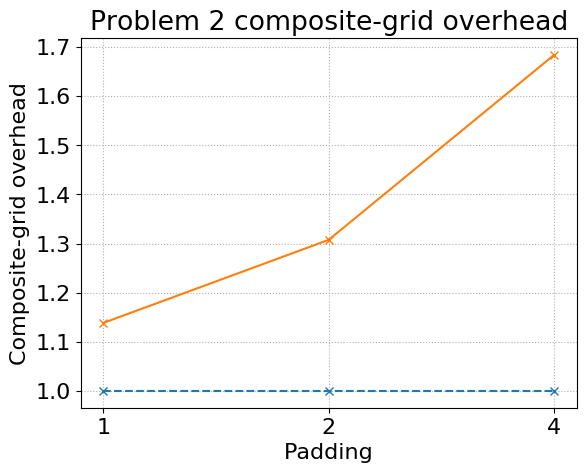
\includegraphics[height=0.3\textwidth]{../figures/gridSizePadProb2}
%
%\end{frame}
%
%% Slide
%\begin{frame}{Algebraic multigrid domain decomposition (AMG-DD)}
%\begin{block}{Padding}
%Larger padding yields:
%\begin{itemize}
%   \item Better accuracy to the global problem
%   \item Larger composite grids
%   \item More communication and computation
%\end{itemize}
%\end{block}
%
%\centering
%\vspace{0.5 cm}
%\includegraphics[height=0.3\textwidth]{../figures/solveNumMessagesByLevel0}
%\includegraphics[height=0.3\textwidth]{../figures/solveNumMessagesByLevel2}
%
%\end{frame}
%
%% Slide
%\begin{frame}{Algebraic multigrid domain decomposition (AMG-DD)}
%\begin{block}{Padding}
%Larger padding yields:
%\begin{itemize}
%   \item Better accuracy to the global problem
%   \item Larger composite grids
%   \item More communication and computation
%\end{itemize}
%\end{block}
%
%\centering
%\vspace{0.5 cm}
%\includegraphics[height=0.3\textwidth]{../figures/solveVolumeByLevel0}
%\includegraphics[height=0.3\textwidth]{../figures/solveVolumeByLevel2}
%
%\end{frame}

% Slide
\begin{frame}{Algebraic multigrid domain decomposition (AMG-DD)}
\begin{block}{Padding}
Accuracy per cost:
\begin{itemize}
   \item Computation
   \item Communication (number of messages and volume)
\end{itemize}
\end{block}

\centering
\vspace{0.5 cm}
% \includegraphics[height=0.3\textwidth]{../figures/resConvByComputation0}
% \includegraphics[height=0.3\textwidth]{../figures/resConvByComputation2}

\end{frame}

% Slide
\begin{frame}{Algebraic multigrid domain decomposition (AMG-DD)}
\begin{block}{Padding}
Accuracy per cost:
\begin{itemize}
   \item Computation
   \item Communication (number of messages and volume)
\end{itemize}
\end{block}

\centering
\vspace{0.5 cm}
% \includegraphics[height=0.3\textwidth]{../figures/resConvByNumMessages0}
% \includegraphics[height=0.3\textwidth]{../figures/resConvByNumMessages2}

\end{frame}

% Slide
\begin{frame}{Algebraic multigrid domain decomposition (AMG-DD)}
\begin{block}{Padding}
Accuracy per cost:
\begin{itemize}
   \item Computation
   \item Communication (number of messages and volume)
\end{itemize}
\end{block}

\centering
\vspace{0.5 cm}
% \includegraphics[height=0.3\textwidth]{../figures/resConvByVolume0}
% \includegraphics[height=0.3\textwidth]{../figures/resConvByVolume2}

\end{frame}

% Slide
\begin{frame}{Algebraic multigrid domain decomposition (AMG-DD)}
\begin{block}{FAC cycles}
More FAC cycles yield:
\begin{itemize}
   \item Better accuracy to the composite solution
   \item More computation
\end{itemize}
\end{block}

\centering
\vspace{0.5 cm}
% \includegraphics[height=0.3\textwidth]{../figures/resConvFACProb0}
% \includegraphics[height=0.3\textwidth]{../figures/resConvFACProb2}

\end{frame}

% Slide
\begin{frame}{Algebraic multigrid domain decomposition (AMG-DD)}
\begin{block}{FAC cycles}
Accuracy per cost:
\begin{itemize}
   \item Computation
   \item More FAC cycles incur no additional communication
\end{itemize}
\end{block}

\centering
\vspace{0.5 cm}
% \includegraphics[height=0.3\textwidth]{../figures/resConvByComputationFAC0}
% \includegraphics[height=0.3\textwidth]{../figures/resConvByComputationFAC2}

\end{frame}

% Slide
\begin{frame}{Algebraic multigrid domain decomposition (AMG-DD)}
%\begin{block}{Additional considerations}
%\begin{itemize}
%\item Recall that communication is most expensive on coarser grids
%\item Finer grids contribute most to storage and computation overhead
%\item Can start AMG-DD on a coarser level:
%\begin{itemize}
%   \item Significantly reduces overhead 
%   \item Retains most of the communication reduction
%\end{itemize}
%\end{itemize}
%\end{block}


\begin{block}{Hybrid AMG-DD}
\begin{itemize}
\item Recall that communication is most expensive on coarser grids
\item Finer grids contribute most to storage and computation overhead
\item Can start AMG-DD on a coarser level:
\begin{itemize}
   \item Significantly reduces overhead 
   \item Retains most of the communication reduction
\end{itemize}
\end{itemize}
\end{block}

\begin{block}{Weak scaling}
\begin{itemize}
\item 42,000 of 30,500 degrees or freedom per processor up to 4,096 processors
\item Padding 1
\end{itemize}
\end{block}

\end{frame}

% Slide
\begin{frame}{Algebraic multigrid domain decomposition (AMG-DD)}
\begin{block}{Computation/storage overhead}
\begin{itemize}
\item Overhead grows slowly with number of processors
\item Use of hybrid AMG-DD can limit overhead
\end{itemize}
\end{block}

\centering
\vspace{0.5 cm}
% \includegraphics[height=0.3\textwidth]{../figures/gridSizeWeakProb0N40000}
% \includegraphics[height=0.3\textwidth]{../figures/gridSizeWeakProb2N10000}

\end{frame}

% Slide
\begin{frame}{Algebraic multigrid domain decomposition (AMG-DD)}
\begin{block}{Number of messages}
\begin{itemize}
\item Number of messages remains small compared to AMG 
\item Hybrid AMG-DD retains most of the reduction in number of messages
\end{itemize}
\end{block}

\centering
\vspace{0.5 cm}
% \includegraphics[height=0.3\textwidth]{../figures/solveNumMessagesWeakProb0N40000}
% \includegraphics[height=0.3\textwidth]{../figures/solveNumMessagesWeakProb2N10000}

\end{frame}

% Slide
\begin{frame}{Algebraic multigrid domain decomposition (AMG-DD)}
\begin{block}{Communication volume}
\begin{itemize}
\item Communication volume grows  slowly with number of processors
\item Hybrid AMG-DD sends almost as much volume as AMG 
\end{itemize}
\end{block}

\centering
\vspace{0.5 cm}
% \includegraphics[height=0.3\textwidth]{../figures/solveVolumeWeakProb0N40000}
% \includegraphics[height=0.3\textwidth]{../figures/solveVolumeWeakProb2N10000}

\end{frame}

%% Slide
%\begin{frame}{Algebraic multigrid domain decomposition (AMG-DD)}
%\begin{block}{Computing regime}
%\begin{itemize}
%\item AMG-DD has been tested up to 4,096 CPUs
%\item Regime is compute-limited
%\end{itemize}
%\end{block}
%
%\centering
%\vspace{0.5 cm}
%\includegraphics[height=0.3\textwidth]{../figures/AspmvTimeByLevelProb0N40000}
%\includegraphics[height=0.3\textwidth]{../figures/AspmvTimeByLevelProb2N10000}
%
%\end{frame}
%
%% Slide
%\begin{frame}{Algebraic multigrid domain decomposition (AMG-DD)}
%\begin{block}{Computing regime}
%\begin{itemize}
%\item GPU clusters present a more communication-limited environment
%\item AMG-DD can provide speedup even for small number of GPUs
%\item 4 GPUs with 250,000 degrees of freedom per GPU
%\end{itemize}
%\end{block}
%
%\centering
%\vspace{0.5 cm}
%\includegraphics[height=0.3\textwidth]{../figures/AspmvTimeByLevel_gpu_P4}
%
%\end{frame}

% Slide
\begin{frame}{Algebraic multigrid domain decomposition (AMG-DD)}
\begin{block}{Timing runs on CPUs}
\begin{itemize}
\item AMG-DD has been tested up to 4,096 CPUs
\item Regime is compute-limited
\item AMG-DD will not provide speedup in a compute-limited regime
\end{itemize}
\end{block}

\begin{block}{Timing runs on GPUs}
\begin{itemize}
\item GPU clusters present a more communication-limited environment
\item AMG-DD can provide speedup even for small number of GPUs
\end{itemize}
\end{block}

\end{frame}

% Slide
\begin{frame}{Algebraic multigrid domain decomposition (AMG-DD)}
\begin{block}{Computing regime}
\begin{itemize}
\item 4 GPUs with 250,000 degrees of freedom per GPU
   \item Computation is relatively much cheaper
   \item AMG-DD with 2 FAC cycles provides greatest speedup
\end{itemize}
\end{block}

\centering
\vspace{0.5 cm}
% \includegraphics[height=0.3\textwidth]{../figures/resConvByTime_gpu_N100}

\end{frame}



% %%%%%%%%%%%%%%%%%%%%%%%%%%%%%%%%%%%%%%%%%%%%%%%%%%%%%%%%%%%%%%%%%%%%%%%%%%%%%%%%%%%%%%%%%%%%%%%%%%%%%%%%%%%%%%%%
\section{Conclusions}

% Slide
\begin{frame}{Conclusions}
\begin{block}{Conclusions}
\begin{itemize}
\item The cost of communication is a significant bottleneck for future scalability of AMG
\item AMG-DD is a promising low-communication alternative to AMG
\item AMG-DD achieves:
\begin{itemize}
\item Small storage and computation overhead compared to AMG
\item Similar or better convergence per iteration compared to AMG
\item Large reduction in both number of messages and communication volume compared to AMG
\item Better accuracy per communication cost than AMG
\item Demonstrated speedup in the right computational regime
\end{itemize}
\end{itemize}
\end{block}
\end{frame}

% Slide
\begin{frame}{Conclusions}
\begin{block}{Future work}
\begin{itemize}
\item Run timing runs on larger GPU clusters
\item Use of stronger smoothers such as tridiagonal solvers
\item Use of mixed precision
\item Communication hiding and asynchronous AMG-DD
\item AMG-DD for non-symmetric problems
\item Application of a DD-like algorithm to multigrid reduction in time (MGRIT)
\end{itemize}
\end{block}

\end{frame}


%%%%%%%%%%%%%%%%%%%%%%%%%%%%%%%%%%%%%%%%%%%%%%%%%%%%%%%%%%%%%%%%%%%%%%%%%%%%%%%%

\end{document}

